\pdfoutput=1% forces arxiv to use pdflatex
% ---------------------------------------------------------------------------------------
\def\Title{Deriving the BSSN equations from the ADM equations}
\def\Author{Leo Brewin}
% ---------------------------------------------------------------------------------------
\documentclass[12pt]{cdblatex}
\usepackage[final]{pdfpages}

\hypersetup{colorlinks=true,
            citecolor=blue,
            linkcolor=red,
            pdfauthor= \Author,
            pdftitle = \Title}

\begin{document}

\CdbSetup{action=verbatim}

\def\Date{2 Jun 2024}

\documentclass[12pt]{cdblatex}
\usepackage{eqtns}
\usepackage{headfoot}

\begin{document}

\section*{PhysRevD.62.044034 equation (9)}

\begin{cadabra}
   from shared import *
   import cdblib

   jsonfile = 'eqtn09.json'
   cdblib.create (jsonfile)

   DgijDt = cdblib.get ('adm.DgijDt','adm.json')
   DhijDt = cdblib.get ('adm.DhijDt','adm.json')

   DphiDt = cdblib.get ('DphiDt','eqtn10.json')

   # --------------------------------------------------------------------------

   gBarij := gBar_{i j} -> \exp(-4\phi) g_{i j}.         # prd62 eqn 05

   Kij    := K_{i j} -> A_{i j} + (1/3) g_{i j} trK.     # prd62 eqn 07

   A2ABar := \exp(-4\phi) A_{i j} -> ABar_{i j}.         # prd62 eqn 08

   # --------------------------------------------------------------------------
   # dgBar_{ij}/dt

   dotgBarij := \partial_{t}{gBar_{i j}}.          # cdb (eq09.101,dotgBarij)

   substitute   (dotgBarij, gBarij)                # cdb (eq09.102,dotgBarij)
   product_rule (dotgBarij)                        # cdb (eq09.103,dotgBarij)
   substitute   (dotgBarij, dexp)                  # cdb (eq09.104,dotgBarij)
   substitute   (dotgBarij, DgijDt)                # cdb (eq09.105,dotgBarij)
   substitute   (dotgBarij, DphiDt)                # cdb (eq09.106,dotgBarij)
   substitute   (dotgBarij, Kij)                   # cdb (eq09.107,dotgBarij)
   distribute   (dotgBarij)                        # cdb (eq09.108,dotgBarij)
   map_sympy    (dotgBarij, "simplify")            # cdb (eq09.109,dotgBarij)
   substitute   (dotgBarij, A2ABar)                # cdb (eq09.110,dotgBarij)

   DgBarijDt := \partial_{t}{gBar_{i j}} -> @(dotgBarij).

   cdblib.put ('dotgBarij',dotgBarij,jsonfile)
\end{cadabra}

\clearpage

\begin{dgroup*}[spread=5pt]
   \begin{dmath*}
      \cdb{eq09.101}
         = \Cdb*{eq09.102}
         = \Cdb*{eq09.103}
         = \Cdb*{eq09.104}
         = \Cdb*{eq09.105}
         = \Cdb*{eq09.106}
         = \Cdb*{eq09.107}
         = \Cdb*{eq09.108}
         = \Cdb*{eq09.109}
         = \Cdb*{eq09.110}
   \end{dmath*}
\end{dgroup*}

\clearpage

\begin{cadabra}
   # --------------------------------------------------------------------------
   # Check against prd62.

   foo := @(dotgBarij).                                # cdb(eq09.lcb,foo)
   bah  = cdblib.get('prd62.eq09.rhs','prd62.json')    # cdb(eq09.prd,bah)

   diff := @(foo) - @(bah).

   diff = product_sort (diff)
   rename_dummies (diff)
   canonicalise   (diff)                               # cdb(eq09.chk,diff)
\end{cadabra}

% \clearpage

\begin{dgroup*}
   \begin{dmath*} \cdb*{eq09.lcb} \end{dmath*}
   \begin{dmath*} \cdb*{eq09.prd} \end{dmath*}
   \begin{dmath*} \cdb*{eq09.chk} \end{dmath*}
\end{dgroup*}

\end{document}

\documentclass[12pt]{cdblatex}
\usepackage{eqtns}
\usepackage{fancyhdr}
\usepackage{footer}

\begin{document}

\section*{PhysRevD.62.044034 equation (10)}

\begin{cadabra}
   from shared import *
   import cdblib

   jsonfile = 'eqtn10.json'
   cdblib.create (jsonfile)

   DgijDt  = cdblib.get ('adm.DgijDt','adm.json')
   DdetgDt = cdblib.get ('adm.DdetgDt','adm.json')

   # --------------------------------------------------------------------------

   phi   := \phi -> (1/12) \log(detg).
   gdotK := g^{i j} K_{i j} -> trK.

   # --------------------------------------------------------------------------
   # d\phi/dt

   dotphi := \partial_{t}{\phi}.     # cdb (eq10.101,dotphi)

   substitute (dotphi, phi)          # cdb (eq10.102,dotphi)
   substitute (dotphi, dlog)         # cdb (eq10.103,dotphi)
   substitute (dotphi, DdetgDt)      # cdb (eq10.104,dotphi)
   substitute (dotphi, DgijDt)       # cdb (eq10.105,dotphi)
   substitute (dotphi, gdotK)        # cdb (eq10.106,dotphi)
   map_sympy  (dotphi, "simplify")   # cdb (eq10.107,dotphi)

   DphiDt := \partial_{t}{\phi} -> @(dotphi).

   cdblib.put ('DphiDt',DphiDt,jsonfile)
\end{cadabra}

\clearpage

\begin{dgroup*}[spread=5pt]
   \begin{dmath*}
      \cdb{eq10.101}
         = \Cdb*{eq10.102}
         = \Cdb*{eq10.103}
         = \Cdb*{eq10.104}
         = \Cdb*{eq10.105}
         = \Cdb*{eq10.106}
         = \Cdb*{eq10.107}
   \end{dmath*}
\end{dgroup*}

\clearpage

\begin{cadabra}
   # --------------------------------------------------------------------------
   # Check against prd62.

   foo := @(dotphi).                                  # cdb(eq10.lcb,foo)
   bah  = cdblib.get('prd62.eq10.rhs','prd62.json')   # cdb(eq10.prd,bah)

   diff := @(foo) - @(bah).

   diff = product_sort (diff)
   rename_dummies (diff)
   canonicalise   (diff)                              # cdb(eq10.chk,diff)
\end{cadabra}

% \clearpage

\begin{dgroup*}
   \begin{dmath*} \cdb*{eq10.lcb} \end{dmath*}
   \begin{dmath*} \cdb*{eq10.prd} \end{dmath*}
   \begin{dmath*} \cdb*{eq10.chk} \end{dmath*}
\end{dgroup*}

\end{document}

\def\Date{2 Jun 2024}

\documentclass[12pt]{cdblatex}
\usepackage{eqtns}
\usepackage{headfoot}

\begin{document}

\section*{PhysRevD.62.044034 equation (11)}

\begin{cadabra}
   from shared import *
   import cdblib

   jsonfile = 'eqtn11.json'
   cdblib.create (jsonfile)

   DhijDt = cdblib.get ('adm.DhijDt','adm.json')
   DKijDt = cdblib.get ('adm.DKijDt','adm.json')

   # --------------------------------------------------------------------------

   trK    := trK -> g^{i j} K_{i j}.
   gdotK  := g^{i j} K_{i j} -> trK.

   Kup := g^{i a} g^{j b} K_{i j} -> K^{a b}.

   Ham := g^{i j} R_{i j} -> K_{i j} K^{i j} - trK trK.

   Kij := K_{i j} -> A_{i j} + (1/3) g_{i j} trK.   # prd62 eqn 07
   Lij := K^{i j} -> A^{i j} + (1/3) g^{i j} trK.   # prd62 eqn 07

   trA1 := A_{i j} g^{i j} -> 0.                    # Aij is trace free
   trA2 := A^{i j} g_{i j} -> 0.

   Asq := A_{i j} A^{i j} -> ABar_{i j} ABar^{i j}.

   gdotg := g_{i j} g^{i j} -> 3.

   # --------------------------------------------------------------------------
   # dK/dt

   dotK := \partial_{t}{trK}.          # cdb (eq11.101,dotK)

   substitute     (dotK,trK)           # cdb (eq11.102,dotK)
   product_rule   (dotK)               # cdb (eq11.103,dotK)
   substitute     (dotK,DhijDt)        # cdb (eq11.104,dotK)
   substitute     (dotK,DKijDt)        # cdb (eq11.105,dotK)
   distribute     (dotK)               # cdb (eq11.106,dotK)
   substitute     (dotK,gdotK)         # cdb (eq11.107,dotK)
   substitute     (dotK,Kup)           # cdb (eq11.108,dotK)
   dotK = product_sort (dotK)          # cdb (eq11.109,dotK)
   substitute     (dotK,Ham)           # cdb (eq11.110,dotK)
   distribute     (dotK)               # cdb (eq11.111,dotK)
   substitute     (dotK,Kij)           # cdb (eq11.112,dotK)
   substitute     (dotK,Lij)           # cdb (eq11.113,dotK)
   distribute     (dotK)               # cdb (eq11.114,dotK)
   substitute     (dotK,trA1)          # cdb (eq11.115,dotK)
   substitute     (dotK,trA2)          # cdb (eq11.116,dotK)
   substitute     (dotK,Asq)           # cdb (eq11.117,dotK)
   substitute     (dotK,gdotg)         # cdb (eq11.118,dotK)
   map_sympy      (dotK, "simplify")   # cdb (eq11.119,dotK)

   DKDt := \partial_{t}{trK} -> @(dotK).

   cdblib.put ('DKDt',DKDt,jsonfile)
\end{cadabra}

\clearpage

\begin{dgroup*}[spread=5pt]
   \begin{dmath*}
      \cdb{eq11.101}
         = \Cdb*{eq11.102}
         = \Cdb*{eq11.103}
         = \Cdb*{eq11.104}
         = \Cdb*{eq11.105}
         = \Cdb*{eq11.106}
         = \Cdb*{eq11.107}
         = \Cdb*{eq11.108}
         = \Cdb*{eq11.109}
         = \Cdb*{eq11.110}
         = \Cdb*{eq11.111}
         = \Cdb*{eq11.112}
         = \Cdb*{eq11.113}
         = \Cdb*{eq11.114}
         = \Cdb*{eq11.115}
         = \Cdb*{eq11.116}
         = \Cdb*{eq11.117}
         = \Cdb*{eq11.118}
         = \Cdb*{eq11.119}
   \end{dmath*}
\end{dgroup*}

\clearpage

\begin{cadabra}
   # --------------------------------------------------------------------------
   # Check against prd62.

   foo := @(dotK).                                      # cdb(eq11.lcb,foo)
   bah  = cdblib.get('prd62.eq11.rhs','prd62.json')     # cdb(eq11.prd,bah)

   diff := @(foo) - @(bah).

   distribute     (diff)
   diff = product_sort (diff)
   rename_dummies (diff)
   map_sympy      (diff, "simplify")
   canonicalise   (diff)                                # cdb(eq11.chk,diff)
\end{cadabra}

% \clearpage

\begin{dgroup*}
   \begin{dmath*} \cdb*{eq11.lcb} \end{dmath*}
   \begin{dmath*} \cdb*{eq11.prd} \end{dmath*}
   \begin{dmath*} \cdb*{eq11.chk} \end{dmath*}
\end{dgroup*}

\end{document}

\documentclass[12pt]{cdblatex}
\usepackage{eqtns}
\usepackage{fancyhdr}
\usepackage{footer}

\begin{document}

\section*{PhysRevD.62.044034 equation (12)}

\begin{cadabra}
   from shared import *
   import cdblib

   jsonfile = 'eqtn12.json'
   cdblib.create (jsonfile)

   DgijDt = cdblib.get ('adm.DgijDt','adm.json')
   DKijDt = cdblib.get ('adm.DKijDt','adm.json')

   DphiDt = cdblib.get ('DphiDt','eqtn10.json')
   DKDt = cdblib.get ('DKDt','eqtn11.json')

   # --------------------------------------------------------------------------
   ABar2A := ABar_{i j} -> \exp(-4\phi) A_{i j}.         # prd62 eqn 08
   A2ABar := A_{i j} -> \exp(4\phi) ABar_{i j}.          # prd62 eqn 08

   Aij    := A_{i j} -> K_{i j} - (1/3) g_{i j} trK.     # prd62 eqn 07
   Kij    := K_{i j} -> A_{i j} + (1/3) g_{i j} trK.     # prd62 eqn 07

   gginv := {g_{i a} g^{a j} -> g_{i}^{j},
             g_{i a} g^{j a} -> g_{i}^{j}}.

   ABarUp := ABar_{i j} g^{j k} -> \exp(-4\phi) ABar_{i}^{k}.

   ABardotABar := ABar_{i j} ABar^{i j} ->
                  (K_{i j}-(1/3)g_{i j} trK) (K^{i j}-(1/3)g^{i j} trK).

   trg := g_{i j} g^{i j} -> 3.

   trK := {K_{i j} g^{i j} -> trK,
           K^{i j} g_{i j} -> trK}.

   Ham := trK**2 -> K_{i j} K^{i j} - g^{i j} R_{i j}.

   # --------------------------------------------------------------------------
   # dABarij/dt

   dotABarij := \partial_{t}{ABar_{i j}}.         # cdb (eq12.101,dotABarij)

   substitute     (dotABarij, ABar2A)             # cdb (eq12.102,dotABarij)
   product_rule   (dotABarij)                     # cdb (eq12.103,dotABarij)
   map_sympy      (dotABarij, "simplify")         # cdb (eq12.104,dotABarij)
   substitute     (dotABarij, DphiDt)             # cdb (eq12.105,dotABarij)
   substitute     (dotABarij, Aij)                # cdb (eq12.106,dotABarij)
   distribute     (dotABarij)                     # cdb (eq12.107,dotABarij)
   substitute     (dotABarij, DKijDt)             # cdb (eq12.108,dotABarij)
   product_rule   (dotABarij)                     # cdb (eq12.109,dotABarij)
   distribute     (dotABarij)                     # cdb (eq12.110,dotABarij)
   substitute     (dotABarij, DKDt)               # cdb (eq12.111,dotABarij)
   substitute     (dotABarij, DgijDt)             # cdb (eq12.112,dotABarij)
   distribute     (dotABarij)                     # cdb (eq12.113,dotABarij)
   substitute     (dotABarij, Kij)                # cdb (eq12.114,dotABarij)
   distribute     (dotABarij)                     # cdb (eq12.115,dotABarij)
   substitute     (dotABarij, gginv)              # cdb (eq12.116,dotABarij)
   eliminate_kronecker (dotABarij)                # cdb (eq12.117,dotABarij)
   substitute     (dotABarij, A2ABar)             # cdb (eq12.118,dotABarij)
   canonicalise   (dotABarij)                     # cdb (eq12.119,dotABarij)
   substitute     (dotABarij, ABardotABar)        # cdb (eq12.120,dotABarij)
   distribute     (dotABarij)                     # cdb (eq12.121,dotABarij)
   substitute     (dotABarij, trg)                # cdb (eq12.122,dotABarij)
   substitute     (dotABarij, trK)                # cdb (eq12.123,dotABarij)
   map_sympy      (dotABarij, "simplify")         # cdb (eq12.124,dotABarij)
   substitute     (dotABarij, Ham)                # cdb (eq12.125,dotABarij)
   distribute     (dotABarij)                     # cdb (eq12.126,dotABarij)
   dotABarij = product_sort (dotABarij)           # cdb (eq12.127,dotABarij)
   substitute     (dotABarij, ABarUp)             # cdb (eq12.128,dotABarij)
   map_sympy      (dotABarij, "simplify")         # cdb (eq12.129,dotABarij)
   factor_out     (dotABarij,$\exp(-4\phi)$)      # cdb (eq12.130,dotABarij)

   DABarijDt := \partial_{t}{ABar_{ij}} -> @(dotABarij).

   cdblib.put ('DABarijDt',DABarijDt,jsonfile)
\end{cadabra}

\clearpage

\begin{dgroup*}[spread=5pt]
   \begin{dmath*}
      \cdb{eq12.101}
         = \Cdb*{eq12.102}
         = \Cdb*{eq12.103}
         = \Cdb*{eq12.104}
         = \Cdb*{eq12.105}
         = \Cdb*{eq12.106}
         = \Cdb*{eq12.107}
         = \Cdb*[\hskip2cm\hfill]{eq12.108}
         = \Cdb*{eq12.109}
         = \Cdb*{eq12.110}
         = \Cdb*{eq12.111}
         = \Cdb*{eq12.112}
   \end{dmath*}
\end{dgroup*}

\clearpage

\begin{dgroup*}[spread=5pt]
   \begin{dmath*}
      \cdb{eq12.101}
         = \Cdb*[\hskip2cm\hfill]{eq12.113}
         = \Cdb*{eq12.114}
         = \Cdb*{eq12.115}
         = \Cdb*{eq12.116}
         = \Cdb*{eq12.117}
   \end{dmath*}
\end{dgroup*}

\clearpage

\begin{dgroup*}[spread=5pt]
   \begin{dmath*}
      \cdb{eq12.101}
         = \Cdb*{eq12.118}
         = \Cdb*{eq12.119}
         = \Cdb*{eq12.120}
         = \Cdb*{eq12.121}
   \end{dmath*}
\end{dgroup*}

\clearpage

\begin{dgroup*}[spread=5pt]
   \begin{dmath*}
      \cdb{eq12.101}
         = \Cdb*{eq12.122}
         = \Cdb*{eq12.123}
         = \Cdb*{eq12.124}
         = \Cdb*{eq12.125}
         = \Cdb*{eq12.126}
         = \Cdb*[\hskip2cm\hfill]{eq12.127}
   \end{dmath*}
\end{dgroup*}

\clearpage

\begin{dgroup*}[spread=5pt]
   \begin{dmath*}
      \cdb{eq12.101}
         = \Cdb*[\hskip2cm\hfill]{eq12.128}
         = \Cdb*{eq12.129}
         = \Cdb*{eq12.130}
   \end{dmath*}
\end{dgroup*}

\clearpage

\begin{cadabra}
   # --------------------------------------------------------------------------
   # Check against prd62.

   foo := @(dotABarij).                                 # cdb(eq12.lcb,foo)
   bah  = cdblib.get('prd62.eq12.rhs','prd62.json')     # cdb(eq12.prd,bah)

   diff := @(foo) - @(bah).

   foo := ABar_{a}^{b} -> gBar^{b c} ABar_{a c}.
   bah := ABar^{a}_{b} -> gBar^{a c} ABar_{c b}.

   substitute     (diff, foo)
   substitute     (diff, bah)
   distribute     (diff)
   diff = product_sort (diff)
   rename_dummies (diff)
   map_sympy      (diff, "simplify")
   canonicalise   (diff)                                # cdb(eq12.chk,diff)
\end{cadabra}

% \clearpage

\begin{dgroup*}
   \begin{dmath*} \cdb*{eq12.lcb} \end{dmath*}
   \begin{dmath*} \cdb*{eq12.prd} \end{dmath*}
   \begin{dmath*} \cdb*{eq12.chk} \end{dmath*}
\end{dgroup*}

\end{document}

\documentclass[12pt]{cdblatex}
\usepackage{eqtns}

\begin{document}

\section*{PhysRevD.62.044034 equation (15)}

\begin{cadabra}
   from shared import *
   import cdblib

   jsonfile = 'eqtn15.json'
   cdblib.create (jsonfile)

   defG2GBar = cdblib.get ('defG2GBar','gamma.json')

   # --------------------------------------------------------------------------
   # Rphi = the part of Rab from the conformal factor

   Rab := R_{a b}.                                                   # cdb (eq15.101,Rab)

   substitute     (Rab, defRab)                                      # cdb (eq15.102,Rab)
   substitute     (Rab, defRiem)                                     # cdb (eq15.103,Rab)
   substitute     (Rab, defG2GBar)                                   # cdb (eq15.104,Rab)
   distribute     (Rab)                                              # cdb (eq15.105,Rab)
   product_rule   (Rab)                                              # cdb (eq15.106,Rab)
   Rab = product_sort (Rab)                                          # cdb (eq15.107,Rab)
   rename_dummies (Rab)                                              # cdb (eq15.108,Rab)
   canonicalise   (Rab)                                              # cdb (eq15.109,Rab)
   substitute     (Rab, $gBar_{b c} gBar^{c a} -> gBar^{a}_{b}$)
   substitute     (Rab, $\partial_{a}{gBar^{a}_{b}} -> 0$)
   substitute     (Rab, $\partial_{a}{gBar_{b}^{c}} -> 0$)
   substitute     (Rab, $gBar^{a}_{a} -> 3$)
   eliminate_kronecker (Rab)                                         # cdb (eq15.110,Rab)
   Rab = product_sort (Rab)                                          # cdb (eq15.111,Rab)
   rename_dummies (Rab)                                              # cdb (eq15.112,Rab)
   canonicalise   (Rab)                                              # cdb (eq15.113,Rab)
   substitute     (Rab, $gBar_{b c} gBar^{c a} -> gBar^{a}_{b}$)     # cdb (eq15.114,Rab)
   substitute     (Rab, $gBar^{a}_{a} -> 3$)                         # cdb (eq15.115,Rab)
   eliminate_kronecker (Rab)                                         # cdb (eq15.116,Rab)

   # |\clearpage|
   # isolate Rphi from Rab by switching to local RNC

   Rphi := @(Rab).

   substitute (Rphi, $GammaBar^{a}_{b c}->0$)                        # cdb (eq15.117,Rphi)
   substitute (Rphi, $\partial_{a}{gBar_{b c}}->0$)                  # cdb (eq15.118,Rphi)
   substitute (Rphi, $\partial_{a}{gBar^{b c}}->0$)                  # cdb (eq15.119,Rphi)

   substitute (Rphi, $\partial_{a b}{\phi} -> DBar_{a b}{\phi}$)     # cdb (eq15.120,Rphi)
   substitute (Rphi, $\partial_{a}{\phi} -> DBar_{a}{\phi}$)         # cdb (eq15.121,Rphi)

   defRphi := Rphi_{a b} -> @(Rphi).

   cdblib.put ('defRphi',defRphi,jsonfile)
\end{cadabra}

\clearpage

\begin{dgroup*}[spread=5pt]
   \begin{dmath*}
      \cdb{eq15.101}
         = \Cdb*{eq15.102}
         = \Cdb*{eq15.103}
         = \Cdb*[\hskip2.5cm\hfill]{eq15.104}
         = \Cdb*{eq15.105}
         = \Cdb*{eq15.106}
         = \Cdb*{eq15.107}
   \end{dmath*}
\end{dgroup*}

\clearpage

\begin{dgroup*}[spread=5pt]
   \begin{dmath*}
      \cdb{eq15.101}
         = \Cdb*{eq15.108}
         = \Cdb*[\hskip2cm\hfill]{eq15.109}
         = \Cdb*{eq15.110}
         = \Cdb*{eq15.111}
         = \Cdb*{eq15.112}
   \end{dmath*}
\end{dgroup*}

\clearpage

\begin{dgroup*}[spread=5pt]
   \begin{dmath*}
      \cdb{eq15.101}
         = \Cdb*[\hskip2.5cm\hfill]{eq15.113}
         = \Cdb*[\hskip2.5cm\hfill]{eq15.114}
         = \Cdb*{eq15.115}
         = \Cdb*{eq15.116}
   \end{dmath*}
\end{dgroup*}

The above doesn't look much like equation (15). So, what do we do? First note that {\tt (eq15.116)}
represents the full $R_{ab}$, that is, equation (14). To isolate the contributions from $\phi$
we can first set $\bar{\Gamma}$ and its derivatives to zero (which in turn requires setting
$\partial_{a} \bar{g}_{bc}=0$). The result is equation {\tt (eq15.119)} below. Having set
$\bar{\Gamma}$ to zero means that we can replace $\partial$ with $\bar{D}$ leading to equation
{\tt (eq15.121)}. But that is clearly a tensor equation and so by the usual arguments it must be true
in all frames (not just this frame with $\bar{\Gamma}=0$). It's a standard argument and I've
probably overdone the discussion. Anyway, equation {\tt (eq15.121)} is exactly equation $(15)$ from
the paper. Yeah.

\begin{dgroup*}[spread=5pt]
   \begin{dmath*}
      R^{\phi}_{ab}
         = \Cdb*{eq15.117}
         = \Cdb*{eq15.118}
         = \Cdb*{eq15.119}
         = \Cdb*{eq15.120}
         = \Cdb*{eq15.121}
   \end{dmath*}
\end{dgroup*}

\clearpage

\begin{cadabra}
   # --------------------------------------------------------------------------
   # Check against prd62.

   foo := @(Rphi).                                      # cdb(eq15.lcb,foo)
   bah  = cdblib.get('prd62.eq15.rhs','prd62.json')     # cdb(eq15.prd,bah)

   diff := @(foo) - @(bah).

   distribute     (diff)
   diff = product_sort (diff)
   rename_dummies (diff)
   map_sympy      (diff, "simplify")
   canonicalise   (diff)                                # cdb(eq15.chk,diff)
\end{cadabra}

% \clearpage

\begin{dgroup*}
   \begin{dmath*} \cdb*{eq15.lcb} \end{dmath*}
   \begin{dmath*} \cdb*{eq15.prd} \end{dmath*}
   \begin{dmath*} \cdb*{eq15.chk} \end{dmath*}
\end{dgroup*}

\end{document}

\documentclass[12pt]{cdblatex}
\usepackage{eqtns}
\usepackage{fancyhdr}
\usepackage{footer}

\begin{document}

\section*{PhysRevD.62.044034 equation (17)}

\begin{cadabra}
   from shared import *
   import cdblib

   jsonfile = 'eqtn17.json'
   cdblib.create (jsonfile)

   # --------------------------------------------------------------------------
   defGammaBar := GammaBar^{a}_{b c} ->
                  (1/2) gBar^{a e} (   \partial_{b}{gBar_{e c}}
                                     + \partial_{c}{gBar_{b e}}
                                     - \partial_{e}{gBar_{b c}}).

   foo := \partial_{a}{gBar_{b c}} gBar^{i b} gBar^{j c} -> - \partial_{a}{gBar^{i j}}.
   bah := \partial_{a}{gBar_{b c}} gBar^{b c} -> 0.   # follows from det gBar = 1

   # --------------------------------------------------------------------------
   # GiBar

   GiBar := gBar^{j k} GammaBar^{i}_{j k}.            # cdb (eq17.101,GiBar)

   substitute     (GiBar, defGammaBar)                # cdb (eq17.102,GiBar)
   distribute     (GiBar)                             # cdb (eq17.103,GiBar)
   GiBar = product_sort (GiBar)                       # cdb (eq17.104,GiBar)
   rename_dummies (GiBar)                             # cdb (eq17.105,GiBar)
   canonicalise   (GiBar)                             # cdb (eq17.106,GiBar)
   substitute     (GiBar, foo)                        # cdb (eq17.107,GiBar)
   substitute     (GiBar, bah)                        # cdb (eq17.108,GiBar)

   defGiBar := GammaBar^{i} -> @(GiBar).

   cdblib.put ('defGiBar',defGiBar,jsonfile)
\end{cadabra}

\clearpage

\begin{dgroup*}[spread=5pt]
   \begin{dmath*}
      \cdb{eq17.101}
         = \Cdb*{eq17.102}
         = \Cdb*{eq17.103}
         = \Cdb*{eq17.104}
         = \Cdb*{eq17.105}
         = \Cdb*{eq17.106}
         = \Cdb*{eq17.107}
         = \Cdb*{eq17.108}
   \end{dmath*}
\end{dgroup*}

\clearpage

\begin{cadabra}
   # --------------------------------------------------------------------------
   # Check against prd62.

   foo := @(GiBar).                                     # cdb(eq17.lcb,foo)
   bah  = cdblib.get('prd62.eq17.rhs','prd62.json')     # cdb(eq17.prd,bah)

   diff := @(foo) - @(bah).

   distribute     (diff)
   diff = product_sort (diff)
   rename_dummies (diff)
   map_sympy      (diff, "simplify")
   canonicalise   (diff)                                # cdb(eq17.chk,diff)
\end{cadabra}

% \clearpage

\begin{dgroup*}
   \begin{dmath*} \cdb*{eq17.lcb} \end{dmath*}
   \begin{dmath*} \cdb*{eq17.prd} \end{dmath*}
   \begin{dmath*} \cdb*{eq17.chk} \end{dmath*}
\end{dgroup*}

\end{document}

\documentclass[12pt]{cdblatex}
\usepackage{eqtns}

\begin{document}

\section*{PhysRevD.62.044034 equation (18)}

\begin{cadabra}
   from shared import *
   import cdblib

   jsonfile = 'eqtn18.json'
   cdblib.create (jsonfile)

   # --------------------------------------------------------------------------
   # RBar pt.1 = split into two terms

   defGammaBar := GammaBar^{a}_{b c} ->
                  (1/2) gBar^{a e} (   \partial_{b}{gBar_{e c}}
                                     + \partial_{c}{gBar_{b e}}
                                     - \partial_{e}{gBar_{b c}}).

   defRiemBar := RBar^{a}_{b c d} ->
                 \partial_{c}{GammaBar^{a}_{b d}} + GammaBar^{a}_{e c} GammaBar^{e}_{b d}
               - \partial_{d}{GammaBar^{a}_{b c}} - GammaBar^{a}_{e d} GammaBar^{e}_{b c}.

   defRBar := RBar_{a b} -> RBar^{c}_{a c b}.

   RBar := RBar_{a b}.                                                  # cdb(eq18.000,RBar)

   substitute   (RBar, defRBar)                                         # cdb(eq18.001,RBar)
   substitute   (RBar, defRiemBar)                                      # cdb(eq18.002,RBar)
   substitute   (RBar, $GammaBar^{a}_{b a} -> 0$)                       # cdb(eq18.003,RBar)  # follows from det g = 1
   canonicalise (RBar)
\end{cadabra}

\clearpage

\begin{dgroup*}[spread=5pt]
   \begin{dmath*}
      \cdb{eq18.000}
         = \Cdb*{eq18.001}
         = \Cdb*{eq18.002}
         = \Cdb*{eq18.003}
   \end{dmath*}
\end{dgroup*}

From here the computations will be splt into two threads, one for each of the two terms in the above result.

\clearpage

\begin{cadabra}
   # --------------------------------------------------------------------------
   # get tmpA & tmpB from RBar

   GammaBar^{a}_{b c}::Weight(label=numG).
   \partial{#}::WeightInherit(label=all, type=multiplicative).

   tmpA := @(RBar).                                                     # cdb(tmp18.101,tmpA)
   keep_weight (tmpA, $numG=1$)                                         # cdb(tmp18.102,tmpA)  # the derivative terms

   tmpB := @(RBar).
   keep_weight (tmpB, $numG=2$)                                         # cdb(tmp18.103,tmpB)  # the quadrtaic terms
\end{cadabra}

\begin{dgroup*}
   \begin{dmath*} \cdb*{tmp18.101} \end{dmath*}
   \begin{dmath*} \cdb*{tmp18.102} \end{dmath*}
   \begin{dmath*} \cdb*{tmp18.103} \end{dmath*}
\end{dgroup*}

\clearpage

\begin{cadabra}
   # --------------------------------------------------------------------------
   # tmpA pt. 1

   substitute   (tmpA, defGammaBar)                                     # cdb(tmp18.201,tmpA)
   distribute   (tmpA)                                                  # cdb(tmp18.202,tmpA)
   product_rule (tmpA)                                                  # cdb(tmp18.203,tmpA)
   substitute   (tmpA, $\partial_{a}{gBar^{a b}} -> - GammaBar^{b}$)    # cdb(tmp18.204,tmpA)
\end{cadabra}

\begin{dgroup*}[spread=5pt]
   \begin{dmath*}
      \cdb{tmp18.102}
         = \Cdb*{tmp18.201}
         = \Cdb*{tmp18.202}
         = \Cdb*{tmp18.203}
         = \Cdb*{tmp18.204}
   \end{dmath*}
\end{dgroup*}

Notice that this result contains two terms containg second derivatives of $\bar g_{ij}$.
This pair of terms will now be replaced with an expression built from the first derivatives
of $\Gamma^{i}$.

\clearpage

\begin{cadabra}
   # --------------------------------------------------------------------------
   # tmpC

   defGi := GammaBar^{i} -> - \partial_{j}{gBar^{i j}}.

   # lower the indices on gBar^{b c}

   defLowerIndices := \partial_{a}{gBar^{b c}} -> - gBar^{i b} gBar^{j c} \partial_{a}{gBar_{i j}}.

   substitute (defGi, defLowerIndices)

   tmpC := gBar_{a i} \partial_{b}{GammaBar^{i}}
         + gBar_{b i} \partial_{a}{GammaBar^{i}}.                       # cdb(tmp18.301,tmpC)

   saveC := @(tmpC).

   substitute   (tmpC, defGi)                                           # cdb(tmp18.302,tmpC)
   product_rule (tmpC)                                                  # cdb(tmp18.303,tmpC)
   distribute   (tmpC)                                                  # cdb(tmp18.304,tmpC)
   canonicalise (tmpC)                                                  # cdb(tmp18.305,tmpC)
   substitute   (tmpC, $gBar_{a b} gBar^{b c} -> gBar_{a}^{c}$)         # cdb(tmp18.306,tmpC)
   eliminate_kronecker (tmpC)                                           # cdb(tmp18.307,tmpC)

   # foo is the target expression to be moved to the lhs

   foo := gBar^{i j} \partial_{a i}{gBar_{b j}}
        + gBar^{i j} \partial_{b i}{gBar_{a j}} -> X_{a b}.

   # bah helps when rebuilding the equation

   bah := X_{a b} ->
          gBar^{i j} \partial_{a i}{gBar_{b j}}
        + gBar^{i j} \partial_{b i}{gBar_{a j}}.

   substitute (tmpC, foo)                                               # cdb(tmp18.308,tmpC)

   # |\clearpage|
   # rearrange to move the target to the lhs

   tmpE := @(tmpC).
   tmpF := @(tmpC).

   X_{a b}::Weight(label=numX).

   # get the two pieces of the equation
   keep_weight (tmpE, $numX=0$)                                         # cdb(tmp18.309,tmpE)
   keep_weight (tmpF, $numX=1$)                                         # cdb(tmp18.310,tmpF)

   substitute  (tmpF, bah)                                              # cdb(tmp18.311,tmpF)

   # now rebuild with terms reorderd
   tmpG := @(saveC) - @(tmpE).                                          # cdb(tmp18.312,tmpG)

   defTmpSub := @(tmpF) -> @(tmpG).                                     # cdb(tmp18.313,defTmpSub)
\end{cadabra}

\clearpage

\begin{dgroup*}[spread=5pt]
   \begin{dmath*}
      \cdb{tmp18.301}
         = \Cdb*{tmp18.302}
         = \Cdb*{tmp18.303}
         = \Cdb*[\hskip2cm\hfill]{tmp18.304}
         = \Cdb*[\hskip2cm\hfill]{tmp18.305}
         = \Cdb*{tmp18.306}
         = \Cdb*{tmp18.307}
         = \Cdb*{tmp18.308}
   \end{dmath*}
\end{dgroup*}

\begin{dgroup*}[spread=5pt]
   \begin{dmath*}
      \cdb{tmp18.311}
         = \Cdb*{tmp18.310}
         = \Cdb*{tmp18.312}
   \end{dmath*}
\end{dgroup*}

This result will now be applied to the earlier equation {\tt (tmp18.204)}.

\clearpage

\begin{cadabra}
   # --------------------------------------------------------------------------
   # tmpA pt.2 eliminate second partial derivatives of gBar

   canonicalise   (tmpA)                                                # cdb(tmp18.401,tmpA)

   substitute     (tmpA, defTmpSub)                                     # cdb(tmp18.402,tmpA)
   tmpA = product_sort (tmpA)
   rename_dummies (tmpA)
   canonicalise   (tmpA)                                                # cdb(tmp18.403,tmpA)

   foo := gBar^{d e} \partial_{c}{gBar_{e f}} -> - gBar_{e f} \partial_{c}{gBar^{d e}}.
   bah := \partial_{d}{gBar^{d f}} -> - GammaBar^{f}.

   substitute     (tmpA, foo)                                           # cdb(tmp18.404,tmpA)
   substitute     (tmpA, bah)                                           # cdb(tmp18.405,tmpA)

   foo := gBar_{e f} \partial_{a}{gBar^{c f}}  -> - \partial_{a}{gBar_{e f}} gBar^{c f}.

   substitute     (tmpA, foo)                                           # cdb(tmp18.406,tmpA)

   foo := gBar_{b d} gBar^{d e}  -> gBar_{b}^{e}.

   substitute     (tmpA, foo)                                           # cdb(tmp18.407,tmpA)
   eliminate_kronecker (tmpA)                                           # cdb(tmp18.408,tmpA)
   tmpA = product_sort (tmpA)
   rename_dummies (tmpA)
   canonicalise   (tmpA)                                                # cdb(tmp18.409,tmpA)
\end{cadabra}

\clearpage

\begin{dgroup*}[spread=5pt]
   \begin{dmath*}
      \cdb{tmp18.102}
         = \Cdb*{tmp18.401}
         = \Cdb*[\hskip2cm\hfill]{tmp18.402}
         = \Cdb*[\hskip2cm\hfill]{tmp18.403}
         = \Cdb*[\hskip2cm\hfill]{tmp18.404}
         = \Cdb*[\hskip2cm\hfill]{tmp18.405}
         = \Cdb*[\hskip2cm\hfill]{tmp18.406}
         = \Cdb*[\hskip2.5cm\hfill]{tmp18.407}
         = \Cdb*[\hskip2.5cm\hfill]{tmp18.408}
         = \Cdb*{tmp18.409}
   \end{dmath*}
\end{dgroup*}

\clearpage

\begin{cadabra}
   # --------------------------------------------------------------------------
   # tmpB

   substitute     (tmpB, defGammaBar)                                   # cdb(tmp18.501,tmpB)
   distribute     (tmpB)                                                # cdb(tmp18.502,tmpB)
   tmpB = product_sort (tmpB)                                           # cdb(tmp18.503,tmpB)
   rename_dummies (tmpB)                                                # cdb(tmp18.504,tmpB)
   canonicalise   (tmpB)                                                # cdb(tmp18.505,tmpB)
\end{cadabra}

\begin{dgroup*}[spread=5pt]
   \begin{dmath*}
      \cdb{tmp18.103}
         = \Cdb*{tmp18.501}
         = \Cdb*{tmp18.502}
         = \Cdb*{tmp18.503}
         = \Cdb*{tmp18.504}
         = \Cdb*{tmp18.505}
   \end{dmath*}
\end{dgroup*}

\clearpage

\begin{cadabra}
   # --------------------------------------------------------------------------
   # RBar pt.2 = Rebuild Rab from tmpA and tmpB

   RBar := @(tmpA) + @(tmpB).

   canonicalise   (RBar)                                                # cdb(eq18.601,RBar)

   foo := \partial_{a}{gBar^{c d}} -> - gBar^{c i} gBar^{d j} \partial_{a}{gBar_{i j}}.

   substitute     (RBar, foo)
   distribute     (RBar)
   RBar = product_sort (RBar)
   rename_dummies (RBar)
   canonicalise   (RBar)                                               # cdb(eq18.602,RBar)

   foo := \partial_{a}{gBar_{b c}} -> GammaBar_{b c a} + GammaBar_{c b a}.

   substitute     (RBar, foo)                                          # cdb(eq18.603,RBar)
   distribute     (RBar)
   RBar = product_sort (RBar)
   rename_dummies (RBar)
   canonicalise   (RBar)                                               # cdb(eq18.604,RBar)

   foo := GammaBar_{d e f} gBar^{d e} -> 0.

   substitute     (RBar, foo)                                          # cdb(eq18.605,RBar)

   defRab := RBar_{a b} -> @(RBar).
\end{cadabra}

\clearpage

\begin{dgroup*}[spread=5pt]
   \begin{dmath*}
      \cdb{eq18.000}
         = \Cdb*{eq18.003}
         = \Cdb*[\hskip2cm\hfill]{eq18.601}
         = \Cdb*{eq18.602}
         = \Cdb*{eq18.603}
         = \Cdb*{eq18.604}
         = \Cdb*{eq18.605}
   \end{dmath*}
\end{dgroup*}

\clearpage

\begin{cadabra}
   # --------------------------------------------------------------------------
   # Check against prd62.

   foo := @(RBar).                                      # cdb(eq18.lcb,foo)
   bah  = cdblib.get('prd62.eq18.rhs','prd62.json')     # cdb(eq18.prd,bah)

   diff := @(foo) - @(bah).

   distribute     (diff)
   diff = product_sort (diff)
   rename_dummies (diff)
   map_sympy      (diff, "simplify")
   canonicalise   (diff)                                # cdb(eq18.chk,diff)
\end{cadabra}

% \clearpage

\begin{dgroup*}
   \begin{dmath*} \cdb*{eq18.lcb} \end{dmath*}
   \begin{dmath*} \cdb*{eq18.prd} \end{dmath*}
   \begin{dmath*} \cdb*{eq18.chk} \end{dmath*}
\end{dgroup*}

\end{document}

\documentclass[12pt]{cdblatex}
\usepackage{eqtns}

\begin{document}

\section*{PhysRevD.62.044034 equation (19)}

\begin{cadabra}
   from shared import *
   import cdblib

   jsonfile = 'eqtn19.json'
   cdblib.create (jsonfile)

   defGiBar = cdblib.get ('defGiBar','eqtn17.json')

   # --------------------------------------------------------------------------
   # DGiBarDt pt.1

   dotgBar_{a b}::Symmetric.
   dotgBar^{a b}::Symmetric.
   dotgBar{#}::LaTeXForm("{\bar{dg}}").

   dotGiBar := \partial_{t}{GammaBar^{i}}.            # cdb (eq19.101,dotGiBar)

   substitute   (dotGiBar, defGiBar)                  # cdb (eq19.102,dotGiBar)
   substitute   (dotGiBar, $\partial_{t a}{gBar^{i a}} -> \partial_{a}{dotgBar^{i a}}$)
                                                      # cdb (eq19.103,dotGiBar)

   defdotgBarD := dotgBar_{i j} -> -2 N ABar_{i j}.
   defdotgBarU := dotgBar^{i j} ->  2 N ABar^{i j}.
   # defABarD2ABarU := ABar_{i j} -> ABar^{a b} gBar_{a i} gBar_{b j}.

   substitute   (dotGiBar, defdotgBarU )              # cdb (eq19.104,dotGiBar)
   product_rule (dotGiBar)                            # cdb (eq19.105,dotGiBar)

   dotGiBar = product_sort (dotGiBar)                 # cdb (eq19.106,dotGiBar)

   cdblib.put ('dotGiBar',dotGiBar,jsonfile)
\end{cadabra}

\clearpage

\begin{dgroup*}[spread=5pt]
   \begin{dmath*}
      \cdb{eq19.101}
         = \Cdb*{eq19.102}
         = \Cdb*{eq19.103}
         = \Cdb*{eq19.104}
         = \Cdb*{eq19.105}
         = \Cdb*{eq19.106}
   \end{dmath*}
\end{dgroup*}

\clearpage

\begin{cadabra}
   # --------------------------------------------------------------------------
   # Check against prd62.

   foo := @(dotGiBar).                                  # cdb (eq19.lcb,foo)
   bah  = cdblib.get('prd62.eq19.rhs','prd62.json')     # cdb (eq19.prd,bah)

   diff := @(foo) - @(bah).

   distribute     (diff)
   product_rule   (diff)
   diff = product_sort (diff)
   rename_dummies (diff)
   map_sympy      (diff, "simplify")
   canonicalise   (diff)                                # cdb (eq19.chk,diff)
\end{cadabra}

% \clearpage

\begin{dgroup*}
   \begin{dmath*} \cdb*{eq19.lcb} \end{dmath*}
   \begin{dmath*} \cdb*{eq19.prd} \end{dmath*}
   \begin{dmath*} \cdb*{eq19.chk} \end{dmath*}
\end{dgroup*}

\end{document}

\documentclass[12pt]{cdblatex}
\usepackage{eqtns}

\begin{document}

\section*{PhysRevD.62.044034 equation (20)}

\begin{cadabra}
   from shared import *
   import cdblib

   jsonfile = 'eqtn20.json'
   cdblib.create (jsonfile)

   dotGiBar = cdblib.get ('dotGiBar','eqtn19.json')
   defMomSub = cdblib.get ('defMomSub','momentum.json')

   # --------------------------------------------------------------------------
   # DGiBarDt pt.2

   substitute (dotGiBar, defMomSub)      # cdb(eq20.101,dotGiBar)
\end{cadabra}

\documentclass[12pt]{cdblatex}
\usepackage{eqtns}

\begin{document}

\section*{PhysRevD.62.044034 equation (19)}

\begin{cadabra}
   from shared import *
   import cdblib

   jsonfile = 'eqtn19.json'
   cdblib.create (jsonfile)

   defGiBar = cdblib.get ('defGiBar','eqtn17.json')

   # --------------------------------------------------------------------------
   # DGiBarDt pt.1

   dotgBar_{a b}::Symmetric.
   dotgBar^{a b}::Symmetric.
   dotgBar{#}::LaTeXForm("{\bar{dg}}").

   dotGiBar := \partial_{t}{GammaBar^{i}}.            # cdb (eq19.101,dotGiBar)

   substitute   (dotGiBar, defGiBar)                  # cdb (eq19.102,dotGiBar)
   substitute   (dotGiBar, $\partial_{t a}{gBar^{i a}} -> \partial_{a}{dotgBar^{i a}}$)
                                                      # cdb (eq19.103,dotGiBar)

   defdotgBarD := dotgBar_{i j} -> -2 N ABar_{i j}.
   defdotgBarU := dotgBar^{i j} ->  2 N ABar^{i j}.
   # defABarD2ABarU := ABar_{i j} -> ABar^{a b} gBar_{a i} gBar_{b j}.

   substitute   (dotGiBar, defdotgBarU )              # cdb (eq19.104,dotGiBar)
   product_rule (dotGiBar)                            # cdb (eq19.105,dotGiBar)

   dotGiBar = product_sort (dotGiBar)                 # cdb (eq19.106,dotGiBar)

   cdblib.put ('dotGiBar',dotGiBar,jsonfile)
\end{cadabra}

\clearpage

\begin{dgroup*}[spread=5pt]
   \begin{dmath*}
      \cdb{eq19.101}
         = \Cdb*{eq19.102}
         = \Cdb*{eq19.103}
         = \Cdb*{eq19.104}
         = \Cdb*{eq19.105}
         = \Cdb*{eq19.106}
   \end{dmath*}
\end{dgroup*}

\clearpage

\begin{cadabra}
   # --------------------------------------------------------------------------
   # Check against prd62.

   foo := @(dotGiBar).                                  # cdb (eq19.lcb,foo)
   bah  = cdblib.get('prd62.eq19.rhs','prd62.json')     # cdb (eq19.prd,bah)

   diff := @(foo) - @(bah).

   distribute     (diff)
   product_rule   (diff)
   diff = product_sort (diff)
   rename_dummies (diff)
   map_sympy      (diff, "simplify")
   canonicalise   (diff)                                # cdb (eq19.chk,diff)
\end{cadabra}

% \clearpage

\begin{dgroup*}
   \begin{dmath*} \cdb*{eq19.lcb} \end{dmath*}
   \begin{dmath*} \cdb*{eq19.prd} \end{dmath*}
   \begin{dmath*} \cdb*{eq19.chk} \end{dmath*}
\end{dgroup*}

\end{document}


\begin{dgroup*}[spread=5pt]
   \begin{dmath*}
      \cdb{eq19.101}
         = \Cdb*{eq19.106}
         = \Cdb*{eq20.101}
   \end{dmath*}
\end{dgroup*}

\clearpage

\begin{cadabra}
   # --------------------------------------------------------------------------
   # Check against prd62.

   foo := @(dotGiBar).                                  # cdb (eq20.lcb,foo)
   bah  = cdblib.get('prd62.eq20.rhs','prd62.json')     # cdb (eq20.prd,bah)

   diff := @(foo) - @(bah).

   distribute     (diff)
   diff = product_sort (diff)
   rename_dummies (diff)
   map_sympy      (diff, "simplify")
   canonicalise   (diff)                                # cdb (eq20.chk,diff)
\end{cadabra}

% \clearpage

\begin{dgroup*}
   \begin{dmath*} \cdb*{eq20.lcb} \end{dmath*}
   \begin{dmath*} \cdb*{eq20.prd} \end{dmath*}
   \begin{dmath*} \cdb*{eq20.chk} \end{dmath*}
\end{dgroup*}

\end{document}


\documentclass[12pt]{cdblatex}
\usepackage{eqtns}

\begin{document}

\section*{PhysRevD.67.084023 equation (27)}

\begin{cadabra}
   from shared import *
   import cdblib

   jsonfile = 'gamma.json'
   cdblib.create (jsonfile)

   # --------------------------------------------------------------------------
   # Gamma in terms of GammaBar and phi, see prd67 eqn 27

   Gamma := \Gamma^{a}_{b c}.                                        # cdb (eq27.101,Gamma)

   substitute   (Gamma, defGamma)                                    # cdb (eq27.102,Gamma)
   substitute   (Gamma, defG2GBarD)                                  # cdb (eq27.103,Gamma)
   substitute   (Gamma, defG2GBarU)                                  # cdb (eq27.104,Gamma)
   distribute   (Gamma)                                              # cdb (eq27.105,Gamma)
   product_rule (Gamma)                                              # cdb (eq27.106,Gamma)
   substitute   (Gamma, dexp)                                        # cdb (eq27.107,Gamma)
   distribute   (Gamma)                                              # cdb (eq27.108,Gamma)
   map_sympy    (Gamma, "simplify")                                  # cdb (eq27.109,Gamma)

   foo := gBar^{a e} \partial_{e}{gBar_{b c}} ->
          - 2 GammaBar^{a}_{b c}
          + gBar^{a e} \partial_{b}{gBar_{e c}}
          + gBar^{a e} \partial_{c}{gBar_{b e}}.

   substitute (Gamma, foo)                                           # cdb (eq27.110,Gamma)
   substitute (Gamma, $gBar^{a i} gBar_{i b} -> gBar^{a}_{b}$)       # cdb (eq27.111,Gamma)
   substitute (Gamma, $gBar^{a i} gBar_{b i} -> gBar^{a}_{b}$)       # cdb (eq27.112,Gamma)

   defG2GBar :=  \Gamma^{a}_{b c} -> @(Gamma).

   cdblib.put ('defG2GBar',defG2GBar,jsonfile)
\end{cadabra}

\clearpage

\begin{dgroup*}[spread=5pt]
   \begin{dmath*}
      \cdb{eq27.101}
         = \Cdb*{eq27.102}
         = \Cdb*{eq27.103}
         = \Cdb*{eq27.104}
         = \Cdb*{eq27.105}
         = \Cdb*{eq27.106}
         = \Cdb*{eq27.107}
         = \Cdb*{eq27.108}
         = \Cdb*{eq27.109}
         = \Cdb*{eq27.110}
         = \Cdb*{eq27.111}
         = \Cdb*{eq27.112}
   \end{dmath*}
\end{dgroup*}

\clearpage

\begin{cadabra}
   # --------------------------------------------------------------------------
   # Check against prd67.

   foo := @(Gamma).                                     # cdb(prd67.eq27.lcb,foo)
   bah  = cdblib.get('prd67.eq27.rhs','prd67.json')     # cdb(prd67.eq27.prd,bah)

   diff := @(foo) - @(bah).

   distribute     (diff)
   diff = product_sort (diff)
   rename_dummies (diff)
   map_sympy      (diff, "simplify")
   canonicalise   (diff)                                # cdb(prd67.eq27.chk,diff)
\end{cadabra}

% \clearpage

\begin{dgroup*}
   \begin{dmath*} \cdb*{prd67.eq27.lcb} \end{dmath*}
   \begin{dmath*} \cdb*{prd67.eq27.prd} \end{dmath*}
   \begin{dmath*} \cdb*{prd67.eq27.chk} \end{dmath*}
\end{dgroup*}

\end{document}

\documentclass[12pt]{cdblatex}
\usepackage{eqtns}

\begin{document}

\section*{PhysRevD.67.084023 equation (19)}

\begin{cadabra}
   from shared import *
   import cdblib

   jsonfile = 'hamiltonian.json'
   cdblib.create (jsonfile)

   # --------------------------------------------------------------------------
   # Hamiltonian constraint

   Ham := R + K_{a b} g^{a b} K_{c d} g^{c d} - K_{a b} K_{c d} g^{a c} g^{b d}.  # cdb (Ham.101,Ham)

   defK2ABarD := K_{i j} -> \exp(4\phi) ABar_{i j} + (1/3) g_{i j} trK.
   defG2GBarD := g_{a b} -> \exp(4\phi) gBar_{a b}.
   defG2GBarU := g^{a b} -> \exp(-4\phi) gBar^{a b}.

   substitute     (Ham, defK2ABarD)   # cdb (Ham.102,Ham)
   substitute     (Ham, defG2GBarD)   # cdb (Ham.103,Ham)
   substitute     (Ham, defG2GBarU)   # cdb (Ham.104,Ham)
   distribute     (Ham)               # cdb (Ham.105,Ham)
   Ham = product_sort (Ham)           # cdb (Ham.106,Ham)
   rename_dummies (Ham)               # cdb (Ham.107,Ham)
   canonicalise   (Ham)               # cdb (Ham.108,Ham)
   map_sympy      (Ham, "simplify")   # cdb (Ham.109,Ham)

   foo := gBar_{a b} gBar^{a b} -> 3.
   bah := gBar_{a c} gBar^{b c} -> gBar_{a}^{b}.

   substitute (Ham, foo)              # cdb (Ham.110,Ham)
   substitute (Ham, bah)              # cdb (Ham.111,Ham)
   eliminate_kronecker (Ham)          # cdb (Ham.112,Ham)

   foo := gBar_{a b} gBar^{a b} -> 3.
   bah := gBar_{a}^{a} -> 3.
   moo := ABar_{a b} gBar^{a b} -> 0.

   substitute     (Ham, foo)          # cdb (Ham.113,Ham)
   substitute     (Ham, bah)          # cdb (Ham.114,Ham)
   substitute     (Ham, moo)          # cdb (Ham.115,Ham)

   foo := ABar_{c d} gBar^{c a} gBar^{d b} -> ABar^{a b}.

   substitute     (Ham, foo)          # cdb (Ham.116,Ham)
   rename_dummies (Ham)               # cdb (Ham.117,Ham)

   cdblib.put ('Ham',Ham,jsonfile)
\end{cadabra}

\clearpage

\begin{dgroup*}
   \begin{dmath*}
      {\cal H}
          = \Cdb*{Ham.101}
          = \Cdb*[\hskip2cm\hfill]{Ham.102}
          = \Cdb*{Ham.103}
          = \Cdb*{Ham.104}
          = \Cdb*[\hskip2cm\hfill]{Ham.105}
          = \Cdb*{Ham.106}
   \end{dmath*}
\end{dgroup*}

\clearpage

\begin{dgroup*}
   \begin{dmath*}
      {\cal H}
          = \Cdb*[\hskip2cm\hfill]{Ham.107}
          = \Cdb*[\hskip2cm\hfill]{Ham.108}
          = \Cdb*{Ham.109}
          = \Cdb*{Ham.110}
          = \Cdb*{Ham.111}
          = \Cdb*{Ham.112}
          = \Cdb*{Ham.113}
          = \Cdb*{Ham.114}
          = \Cdb*{Ham.115}
          = \Cdb*{Ham.116}
          = \Cdb*{Ham.117}
   \end{dmath*}
\end{dgroup*}

\clearpage

\begin{cadabra}
   # --------------------------------------------------------------------------
   # Check against prd67.

   foo := @(Ham).                                       # cdb(prd67.eq19.lcb,foo)
   bah  = cdblib.get('prd67.eq19.rhs','prd67.json')     # cdb(prd67.eq19.prd,bah)

   diff := @(foo) - @(bah).

   distribute     (diff)
   diff = product_sort (diff)
   rename_dummies (diff)
   map_sympy      (diff, "simplify")
   canonicalise   (diff)                                # cdb(prd67.eq19.chk,diff)
\end{cadabra}

% \clearpage

\begin{dgroup*}
   \begin{dmath*} \cdb*{prd67.eq19.lcb} \end{dmath*}
   \begin{dmath*} \cdb*{prd67.eq19.prd} \end{dmath*}
   \begin{dmath*} \cdb*{prd67.eq19.chk} \end{dmath*}
\end{dgroup*}

\end{document}

\documentclass[12pt]{cdblatex}
\usepackage{eqtns}

\begin{document}

\section*{PhysRevD.67.084023 equation (20)}

\begin{cadabra}
   from shared import *
   import cdblib

   jsonfile = 'momentum.json'

   defG2GBar = cdblib.get ('defG2GBar','gamma.json')

   # --------------------------------------------------------------------------
   # Momentum constraint pt.1

   Mom := D_{j}{K^{i j} - g^{i j} trK}.                                       # cdb(Mom.101,Mom)

   defDgD := D_{a}{g_{b c}} -> 0.
   defDgU := D_{a}{g^{b c}} -> 0.

   defDtrK   := D_{a}{trK} -> \partial_{a}{trK}.
   defDexp   := D_{a}{\exp(-4\phi)} -> -4\exp(-4\phi) \partial_{a}{\phi}.

   distribute   (Mom)                                                         # cdb(Mom.102,Mom)
   product_rule (Mom)                                                         # cdb(Mom.103,Mom)
   substitute   (Mom, defDgU)                                                 # cdb(Mom.104,Mom)

   defK2ABarU := K^{i j} -> \exp(-4\phi) ABar^{i j} + (1/3) g^{i j} trK.

   substitute   (Mom, defK2ABarU)                                             # cdb(Mom.105,Mom)
   distribute   (Mom)                                                         # cdb(Mom.106,Mom)
   product_rule (Mom)                                                         # cdb(Mom.107,Mom)
   substitute   (Mom, defDtrK)                                                # cdb(Mom.108,Mom)
   substitute   (Mom, defDgU)                                                 # cdb(Mom.109,Mom)
   substitute   (Mom, defDexp)                                                # cdb(Mom.110,Mom)

\end{cadabra}

\clearpage

\begin{dgroup*}[spread=5pt]
   \begin{dmath*}
      {\cal D}^{j}
         = \Cdb*{Mom.101}
         = \Cdb*{Mom.102}
         = \Cdb*{Mom.103}
         = \Cdb*{Mom.104}
         = \Cdb*{Mom.105}
         = \Cdb*{Mom.106}
         = \Cdb*{Mom.107}
         = \Cdb*{Mom.108}
         = \Cdb*{Mom.109}
         = \Cdb*{Mom.110}
   \end{dmath*}
\end{dgroup*}

\clearpage

\begin{cadabra}
   # --------------------------------------------------------------------------
   # Momentum constraint pt.2

   confMom := \exp(4\phi) @(Mom).

   defG2GBarU := g^{i j} -> \exp(-4\phi) gBar^{i j}.

   distribute   (confMom)                                                     # cdb(confMom.101,confMom)
   substitute   (confMom, defG2GBarU)                                         # cdb(confMom.102,confMom)
   map_sympy    (confMom, "simplify")                                         # cdb(confMom.103,confMom)

   defDAabU  := D_{a}{ABar^{b c}} ->  \partial_{a}{ABar^{b c}}
                                    + \Gamma^{b}_{i a} ABar^{i c}
                                    + \Gamma^{c}_{i a} ABar^{b i}.

   substitute     (confMom, defDAabU)                                         # cdb(confMom.104,confMom)
   substitute     (confMom, defG2GBar)                                        # cdb(confMom.105,confMom)
   distribute     (confMom)                                                   # cdb(confMom.106,confMom)
   confMom = product_sort (confMom)                                           # cdb(confMom.107,confMom)
   rename_dummies (confMom)                                                   # cdb(confMom.108,confMom)
   canonicalise   (confMom)                                                   # cdb(confMom.109,confMom)
   substitute     (confMom, $gBar^{i}_{i} -> 3$)                              # cdb(confMom.110,confMom)
   substitute     (confMom, $gBar_{i j} ABar^{i j} -> 0$)                     # cdb(confMom.111,confMom)
   substitute     (confMom, $gBar_{a i} gBar^{i b} -> gBar_{a}^{b}$)          # cdb(confMom.112,confMom)
   substitute     (confMom, $GammaBar^{b}_{a b} -> 0$)                        # cdb(confMom.113,confMom) # follows from det gBar = 1
   eliminate_kronecker (confMom)                                              # cdb(confMom.114,confMom)
   rename_dummies (confMom)
   canonicalise   (confMom)                                                   # cdb(confMom.115,confMom)

   cdblib.put ('confMom',confMom,jsonfile)
\end{cadabra}

\clearpage

\begin{dgroup*}[spread=5pt]
   \begin{dmath*}
      \exp(4\phi) {\cal D}^{j}
         = \Cdb*{confMom.101}
         = \Cdb*{confMom.102}
         = \Cdb*{confMom.103}
         = \Cdb*{confMom.104}
         = \Cdb*[\hskip3.0cm\hfill]{confMom.105}
         = \Cdb*[\hskip2.0cm\hfill]{confMom.106}
         = \Cdb*[\hskip2.0cm\hfill]{confMom.107}
         = \Cdb*[\hskip2.0cm\hfill]{confMom.108}
         = \Cdb*[\hskip2.5cm\hfill]{confMom.109}
         = \Cdb*{confMom.110}
         = \Cdb*{confMom.111}
   \end{dmath*}
\end{dgroup*}

\clearpage

\begin{dgroup*}[spread=5pt]
   \begin{dmath*}
      \exp(4\phi) {\cal D}^{j}
         = \Cdb*{confMom.112}
         = \Cdb*{confMom.113}
         = \Cdb*{confMom.114}
         = \Cdb*{confMom.115}
   \end{dmath*}
\end{dgroup*}

\clearpage

\begin{cadabra}
   tmpA := @(confMom).                                              # cdb(confMom.201,tmpA)
   tmpB := @(confMom).

   X^{b c}_{a}::Weight(label=numX).

   Xbca := \partial_{a}{ABar^{b c}}.                                # cdb(confMom.202,Xbca)

   foo := \partial_{a}{ABar^{b c}} -> X^{b c}_{a}.
   bah := X^{b c}_{a} -> \partial_{a}{ABar^{b c}}.

   substitute  (tmpA, foo)                                          # cdb(confMom.203,tmpA)
   substitute  (tmpB, foo)                                          # cdb(confMom.204,tmpB)
   drop_weight (tmpA, $numX=1$)                                     # cdb(confMom.205,tmpA)
   keep_weight (tmpB, $numX=1$)                                     # cdb(confMom.206,tmpB)
   substitute  (tmpB, bah)                                          # cdb(confMom.207,tmpB)

   tmpC := - @(tmpA).                                               # cdb(confMom.208,tmpC)

   defMomSub := @(tmpB) -> @(tmpC).                                 # cdb(confMom.209,defMomSub)

   cdblib.put ('defMomSub',defMomSub,jsonfile)
\end{cadabra}

\clearpage

\begin{dgroup*}
   \begin{dmath*} 0 =  \Cdb*{confMom.201} \end{dmath*}
   \begin{dmath*} 0 =  \Cdb*{confMom.203} \end{dmath*}
   \begin{dmath*}
      \cdb{confMom.202} = \Cdb*{confMom.206}
                        = \Cdb*{confMom.208}
   \end{dmath*}
   \begin{dmath*} \Cdb*{confMom.209} \end{dmath*}
\end{dgroup*}

\clearpage

\begin{cadabra}
   # --------------------------------------------------------------------------
   # Check against prd67.

   foo := @(confMom).                                   # cdb(prd67.eq20.lcb,foo)
   bah  = cdblib.get('prd67.eq20.rhs','prd67.json')     # cdb(prd67.eq20.prd,bah)

   diff := @(foo) - @(bah).

   distribute     (diff)
   diff = product_sort (diff)
   rename_dummies (diff)
   map_sympy      (diff, "simplify")
   canonicalise   (diff)                                # cdb(prd67.eq20.chk,diff)
\end{cadabra}

% \clearpage

\begin{dgroup*}
   \begin{dmath*} \cdb*{prd67.eq20.lcb} \end{dmath*}
   \begin{dmath*} \cdb*{prd67.eq20.prd} \end{dmath*}
   \begin{dmath*} \cdb*{prd67.eq20.chk} \end{dmath*}
\end{dgroup*}

\end{document}


% =======================================================================================
\section*{Deriving the BSSN equations from the ADM equations}

The following Cadabra codes verifies, for the particular case of vacuum spacetimes,
the main equations (with zero-shift) in the Phys Rev D papers Phys.Rev.D. (62) 044034 (2000) and
Phys.Rev.D. (67) 084023 (2003) by Miguel Alcubierre, Bernd Brugmann etal. .

The two papers are abbreviated as pdr62 and prd67 respectively.

All of the essential BSSN equations are covered, in particlular equations
9, 10, 11, 12 , 15, 17, 18, 19 and 20 from prd62 and equations 19, 20 and 27 from
prd67.

The first few pages provides a summary of the calculations. For each equation the
summary is of the form
%
\begin{dgroup*}
   \begin{dmath*} \cdb*{eq18.lcb} \end{dmath*}
   \begin{dmath*} \cdb*{eq18.prd} \end{dmath*}
   \begin{dmath*} \cdb*{eq18.chk} \end{dmath*}
\end{dgroup*}

The first line records the output from the Cadabra code, the second line is the
corresponding equation in prd62 (or prd67) while the third line shows the difference.
The good news is that for each equation the difference is zero (as it should be).

The summary is then followed by the full details of the calculations for each
equation. The output includes all of the steps. The odd looking equation numbers are
tags that match the line in the corresponding Cadabra source. Thus the following
output (from prd62 equation 11)
%
\begin{dgroup*}[spread=5pt]
   \begin{dmath*}
      \cdb{eq11.101}
         = \Cdb*{eq11.102}
         = \Cdb*{eq11.103}
         = \Cdb*{eq11.104}
         = \Cdb*{eq11.105}
   \end{dmath*}
\end{dgroup*}
%
can be matched line-by-line with the Cadabra code
%
\begin{cadabra}[numbers=none]
   substitute     (dotK,trK)           # cdb (eq11.102,dotK)
   product_rule   (dotK)               # cdb (eq11.103,dotK)
   substitute     (dotK,DhijDt)        # cdb (eq11.104,dotK)
   substitute     (dotK,DKijDt)        # cdb (eq11.105,dotK)
\end{cadabra}

\clearpage

% =======================================================================================
\section*{Running the codes}

To run any of the codes you will need to install Cadabra. Compiling and installing
Cadabra is straightforward with full details provided on the
\url{https://github.com/kpeeters/cadabra2.git} repository on GitHub.

You will also need to install the hybrid-latex tools. These are simple scripts and
LaTeX macros that allow the Cadabra output to be caught and integrated back into the
LaTeX source. See the {\tt INSTALL.txt} file in {\tt hybrid-latex} for full details.
The documentation for hybrid-latex tools is included in the {\tt hybrid-latex}
directory.

To compile all of the files in one go just use
\lstset{numbers=none}
\begin{lstlisting}
   cd source
   make
\end{lstlisting}

You can compile any one of the files (e.g., {\tt eqtn11.tex}) using any of the
following (from within the {\tt source} directory)

\lstset{numbers=none}
\begin{lstlisting}
   cdblatex.sh -i eqtn11
   make  eqtn11
   make .eqtn11
\end{lstlisting}

The first two commands will force a recompile of {\tt eqtn11} while the third command
will use the magic of makefiles to determine if it (and its dependencies) needs to be
recompiled.

The {\tt cdblatex.sh} is the main script in the hybrid-latex codes. It does the job of
extracting rhe embedded Cadabra code, running that code through Cadabra, collecting
the output and finally making that output available to the LaTeX source.

You may want to look inside the {\tt Makefile} to see which targets are available.

Note that there are dependencies amongst the files and these dependencies are encoded
in the makefile. See the file {\tt SEQUENCE.txt} for the details.

\clearpage

% =======================================================================================
\section*{PhysRevD.62.044034}

   % --------------------------------------------------
   % Equation 9

   \begin{dgroup*}
      \begin{dmath*} \cdb*{eq09.lcb} \end{dmath*}
      \begin{dmath*} \cdb*{eq09.prd} \end{dmath*}
      \begin{dmath*} \cdb*{eq09.chk} \end{dmath*}
   \end{dgroup*}

   % --------------------------------------------------
   % Equation 10

   \begin{dgroup*}
      \begin{dmath*} \cdb*{eq10.lcb} \end{dmath*}
      \begin{dmath*} \cdb*{eq10.prd} \end{dmath*}
      \begin{dmath*} \cdb*{eq10.chk} \end{dmath*}
   \end{dgroup*}

   % --------------------------------------------------
   % Equation 11

   \begin{dgroup*}
      \begin{dmath*} \cdb*{eq11.lcb} \end{dmath*}
      \begin{dmath*} \cdb*{eq11.prd} \end{dmath*}
      \begin{dmath*} \cdb*{eq11.chk} \end{dmath*}
   \end{dgroup*}

   % --------------------------------------------------
   % Equation 12

   \begin{dgroup*}
      \begin{dmath*} \cdb*{eq12.lcb} \end{dmath*}
      \begin{dmath*} \cdb*{eq12.prd} \end{dmath*}
      \begin{dmath*} \cdb*{eq12.chk} \end{dmath*}
   \end{dgroup*}

   % --------------------------------------------------
   % Equation 15

   \begin{dgroup*}
      \begin{dmath*} \cdb*{eq15.lcb} \end{dmath*}
      \begin{dmath*} \cdb*{eq15.prd} \end{dmath*}
      \begin{dmath*} \cdb*{eq15.chk} \end{dmath*}
   \end{dgroup*}

   % --------------------------------------------------
   % Equation 17

   \begin{dgroup*}
      \begin{dmath*} \cdb*{eq17.lcb} \end{dmath*}
      \begin{dmath*} \cdb*{eq17.prd} \end{dmath*}
      \begin{dmath*} \cdb*{eq17.chk} \end{dmath*}
   \end{dgroup*}

   % --------------------------------------------------
   % Equation 18

   \begin{dgroup*}
      \begin{dmath*} \cdb*{eq18.lcb} \end{dmath*}
      \begin{dmath*} \cdb*{eq18.prd} \end{dmath*}
      \begin{dmath*} \cdb*{eq18.chk} \end{dmath*}
   \end{dgroup*}

   % --------------------------------------------------
   % Equation 19

   \begin{dgroup*}
      \begin{dmath*} \cdb*{eq19.lcb} \end{dmath*}
      \begin{dmath*} \cdb*{eq19.prd} \end{dmath*}
      \begin{dmath*} \cdb*{eq19.chk} \end{dmath*}
   \end{dgroup*}

   % --------------------------------------------------
   % Equation 20

   \begin{dgroup*}
      \begin{dmath*} \cdb*{eq20.lcb} \end{dmath*}
      \begin{dmath*} \cdb*{eq20.prd} \end{dmath*}
      \begin{dmath*} \cdb*{eq20.chk} \end{dmath*}
   \end{dgroup*}

% =======================================================================================
\section*{PhysRevD.67.084023}

   % --------------------------------------------------
   % Equation 19

   \begin{dgroup*}
      \begin{dmath*} \cdb*{prd67.eq19.lcb} \end{dmath*}
      \begin{dmath*} \cdb*{prd67.eq19.prd} \end{dmath*}
      \begin{dmath*} \cdb*{prd67.eq19.chk} \end{dmath*}
   \end{dgroup*}

   % --------------------------------------------------
   % Equation 20

   \begin{dgroup*}
      \begin{dmath*} \cdb*{prd67.eq20.lcb} \end{dmath*}
      \begin{dmath*} \cdb*{prd67.eq20.prd} \end{dmath*}
      \begin{dmath*} \cdb*{prd67.eq20.chk} \end{dmath*}
   \end{dgroup*}

   % --------------------------------------------------
   % Equation 27

   \begin{dgroup*}
      \begin{dmath*} \cdb*{prd67.eq27.lcb} \end{dmath*}
      \begin{dmath*} \cdb*{prd67.eq27.prd} \end{dmath*}
      \begin{dmath*} \cdb*{prd67.eq27.chk} \end{dmath*}
   \end{dgroup*}

\clearpage

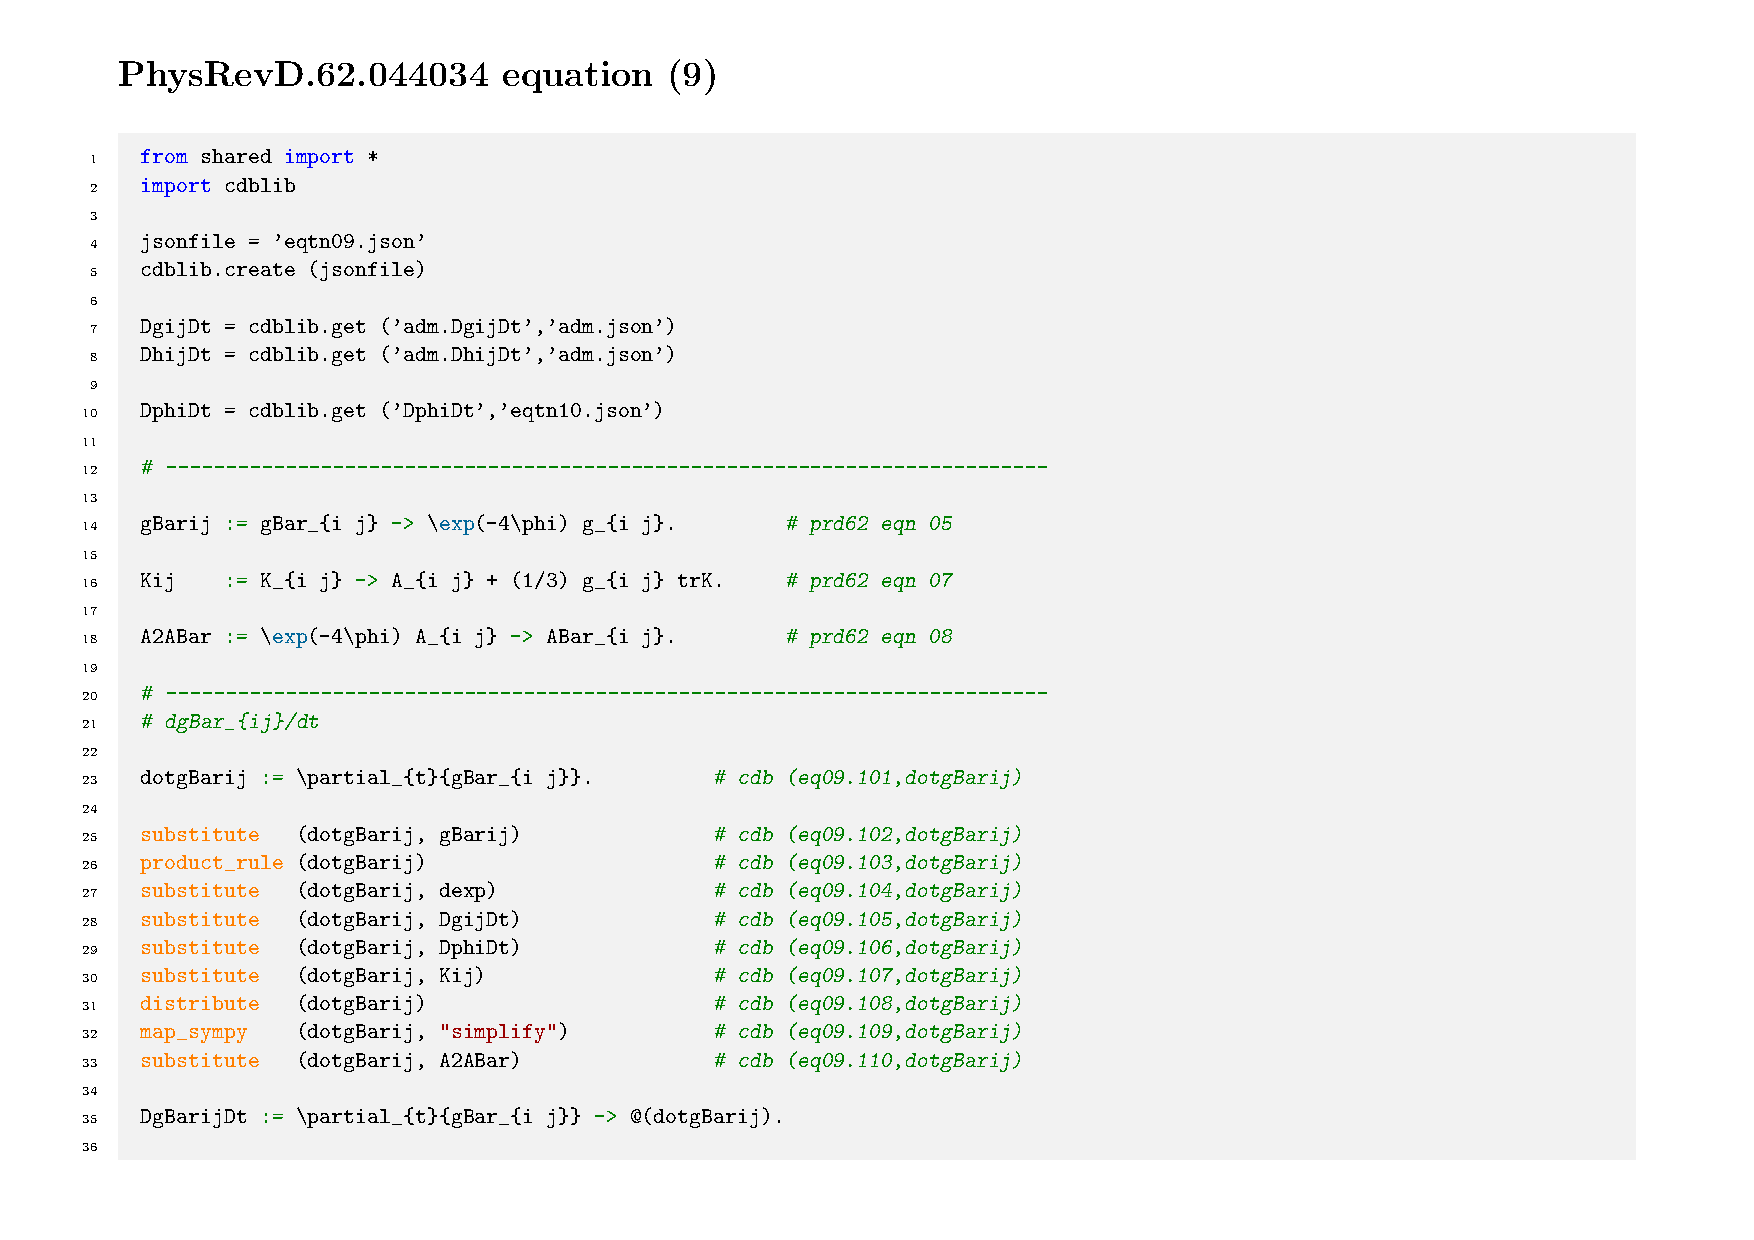
\includepdf[pages=1-]{./eqtn09.pdf}
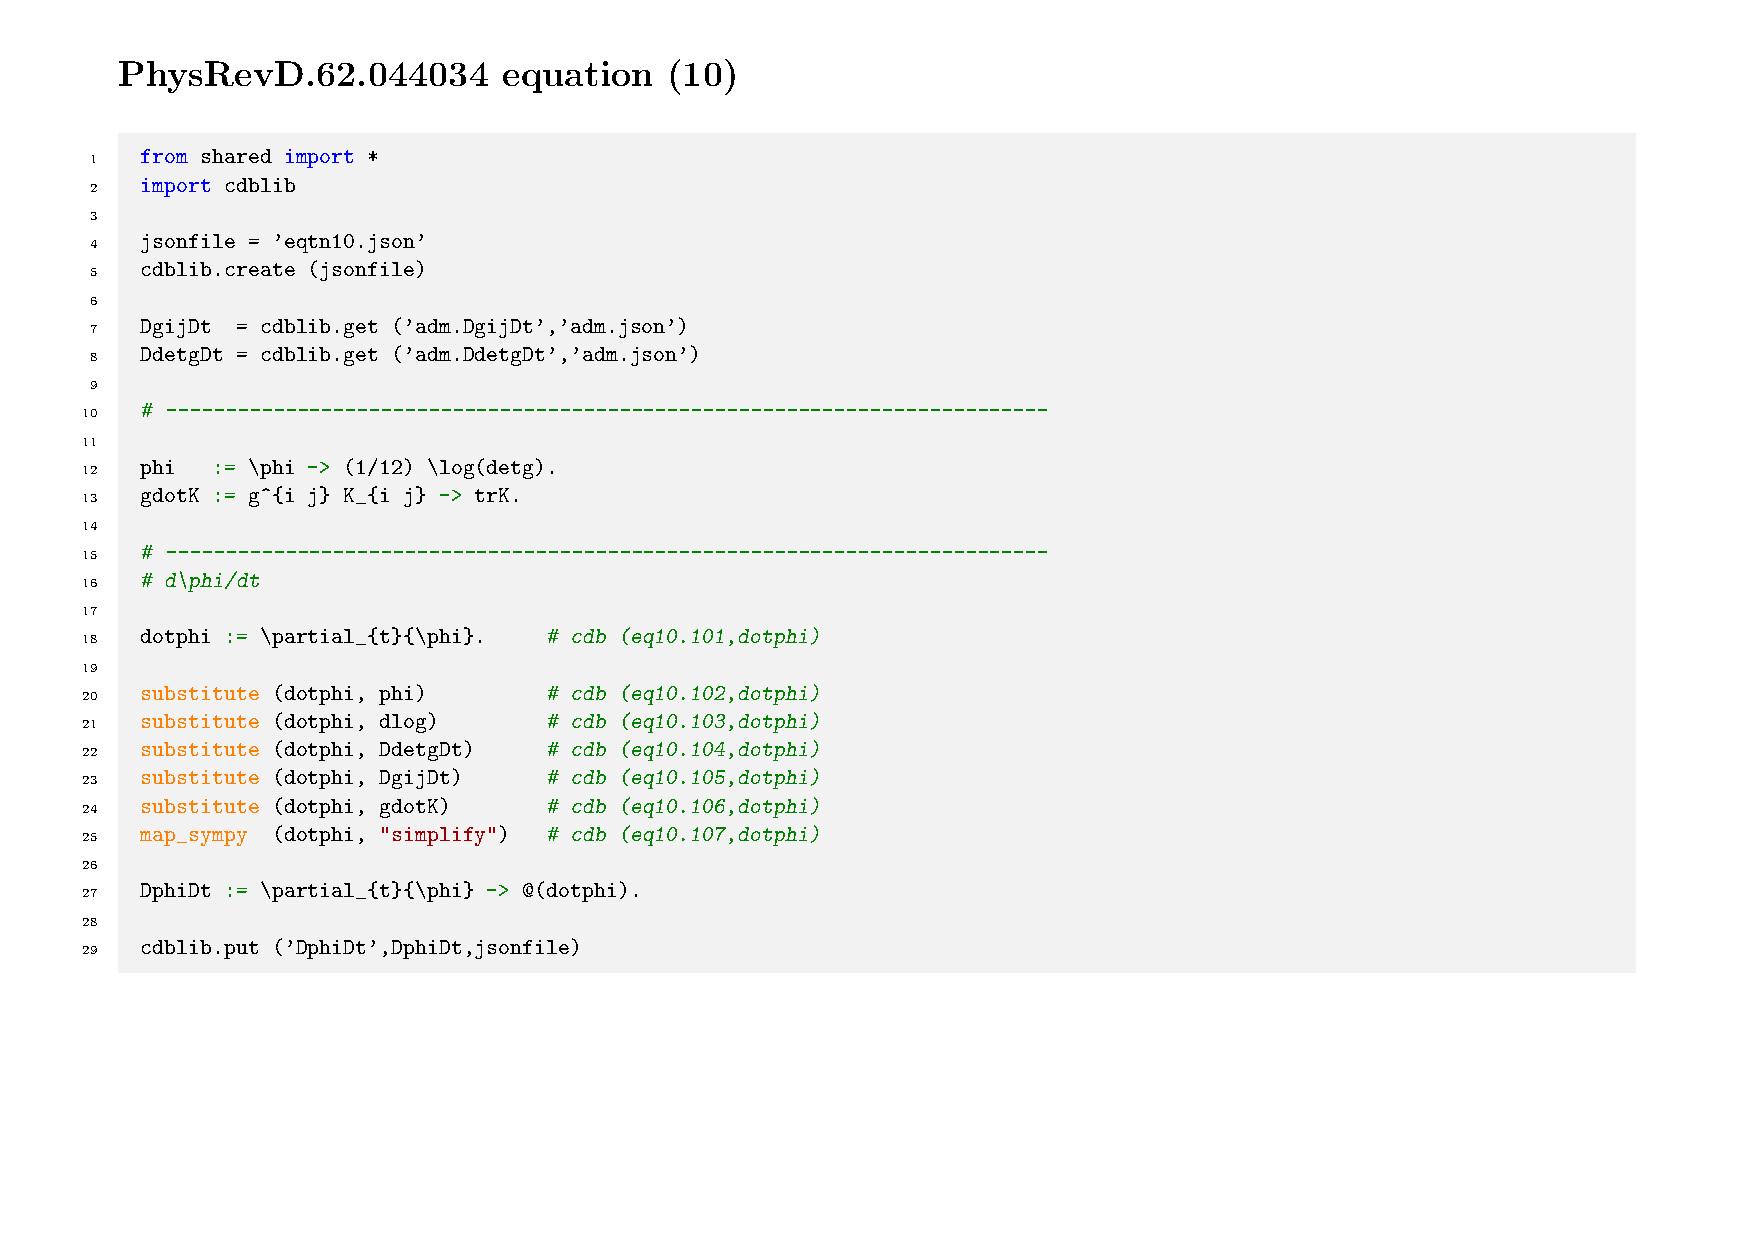
\includepdf[pages=1-]{./eqtn10.pdf}
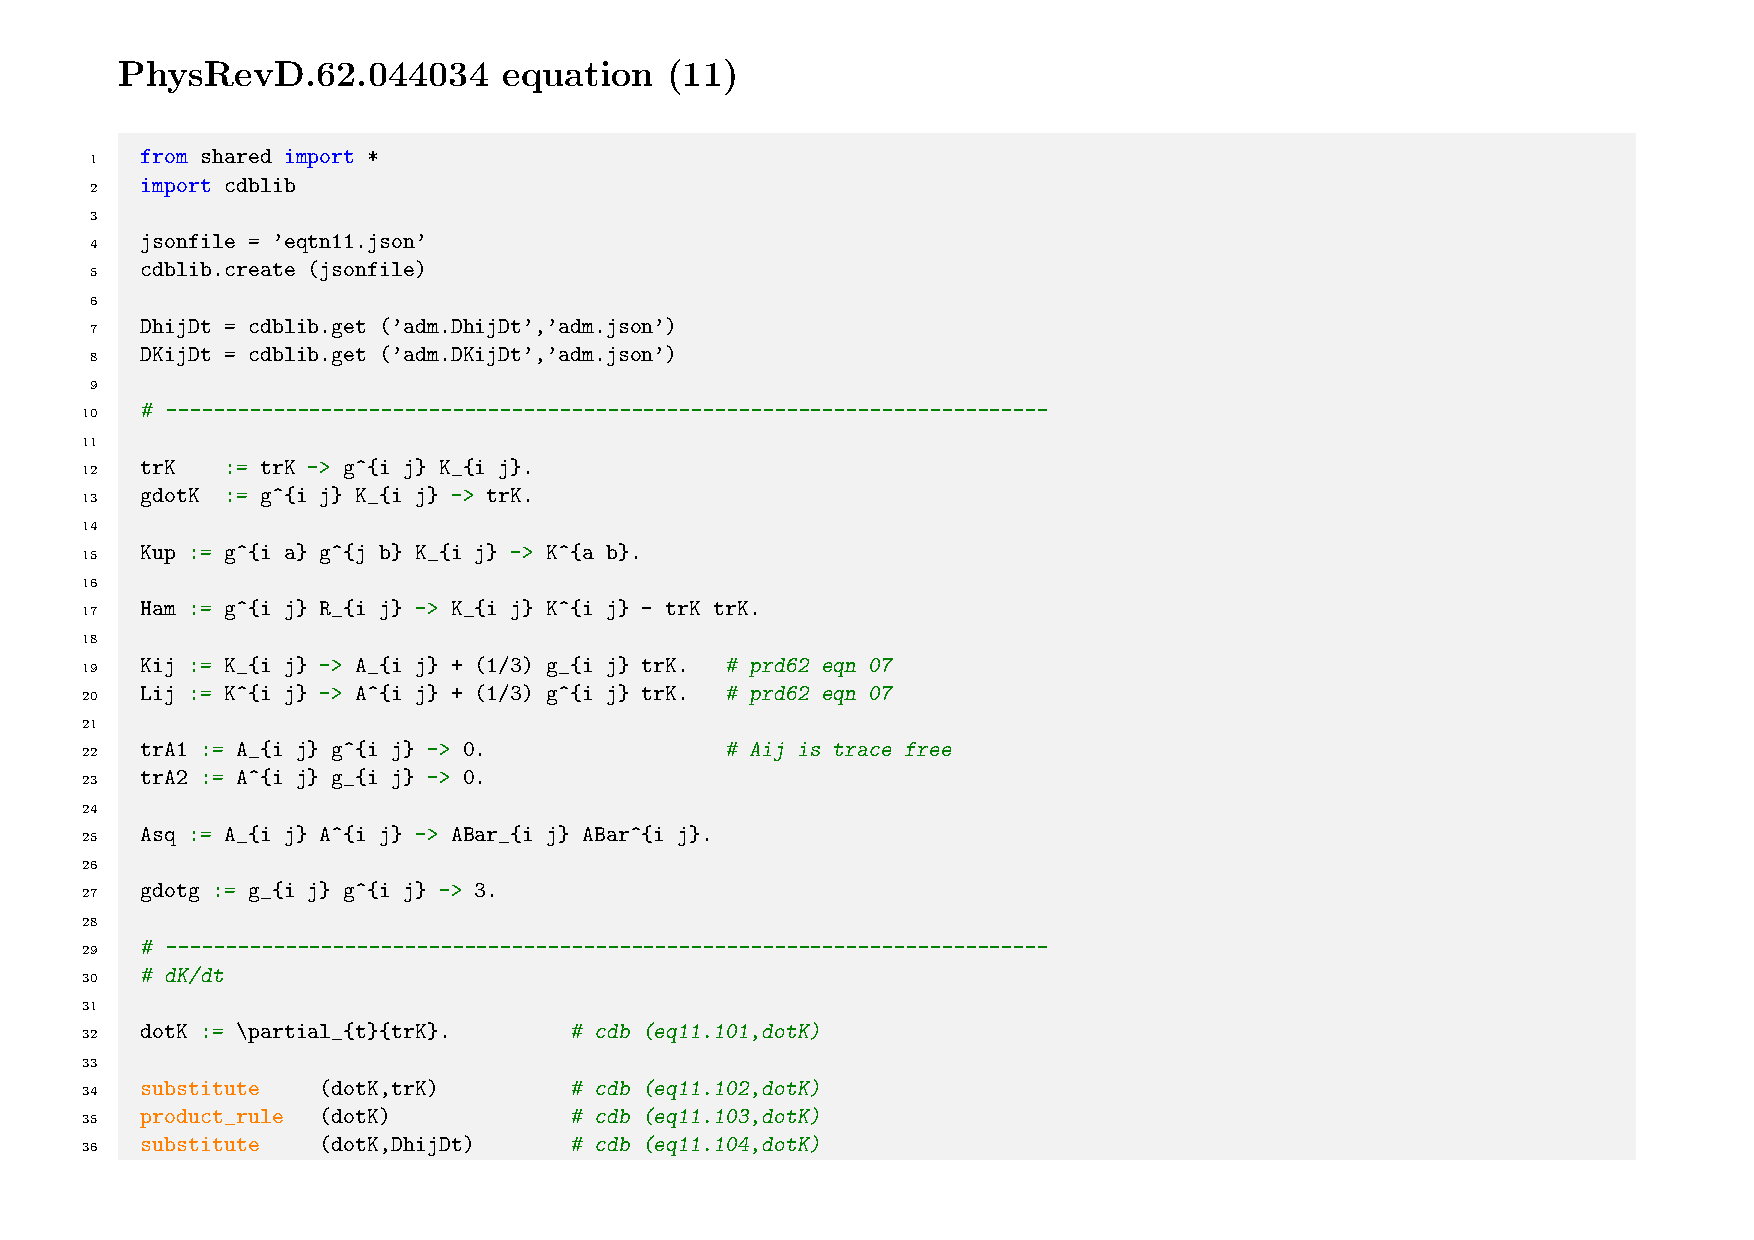
\includepdf[pages=1-]{./eqtn11.pdf}
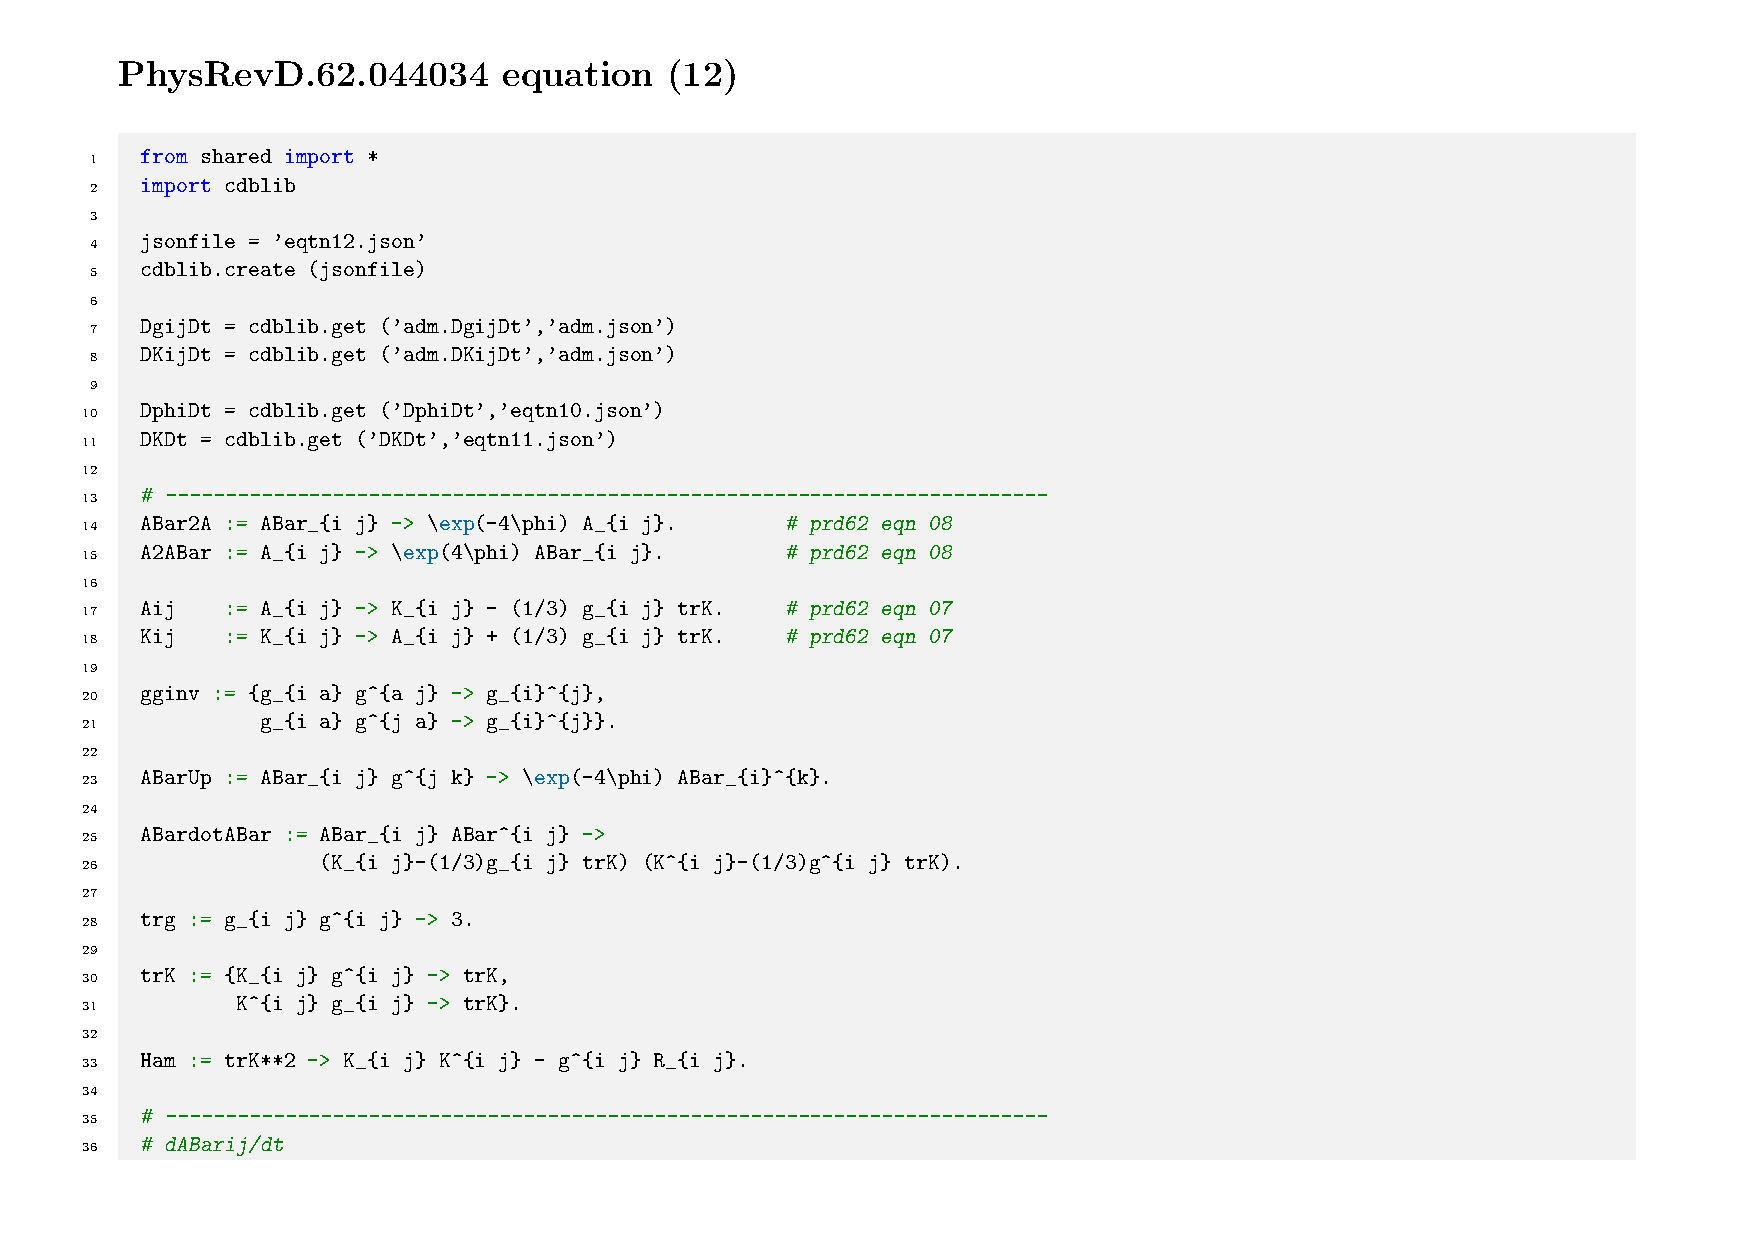
\includepdf[pages=1-]{./eqtn12.pdf}
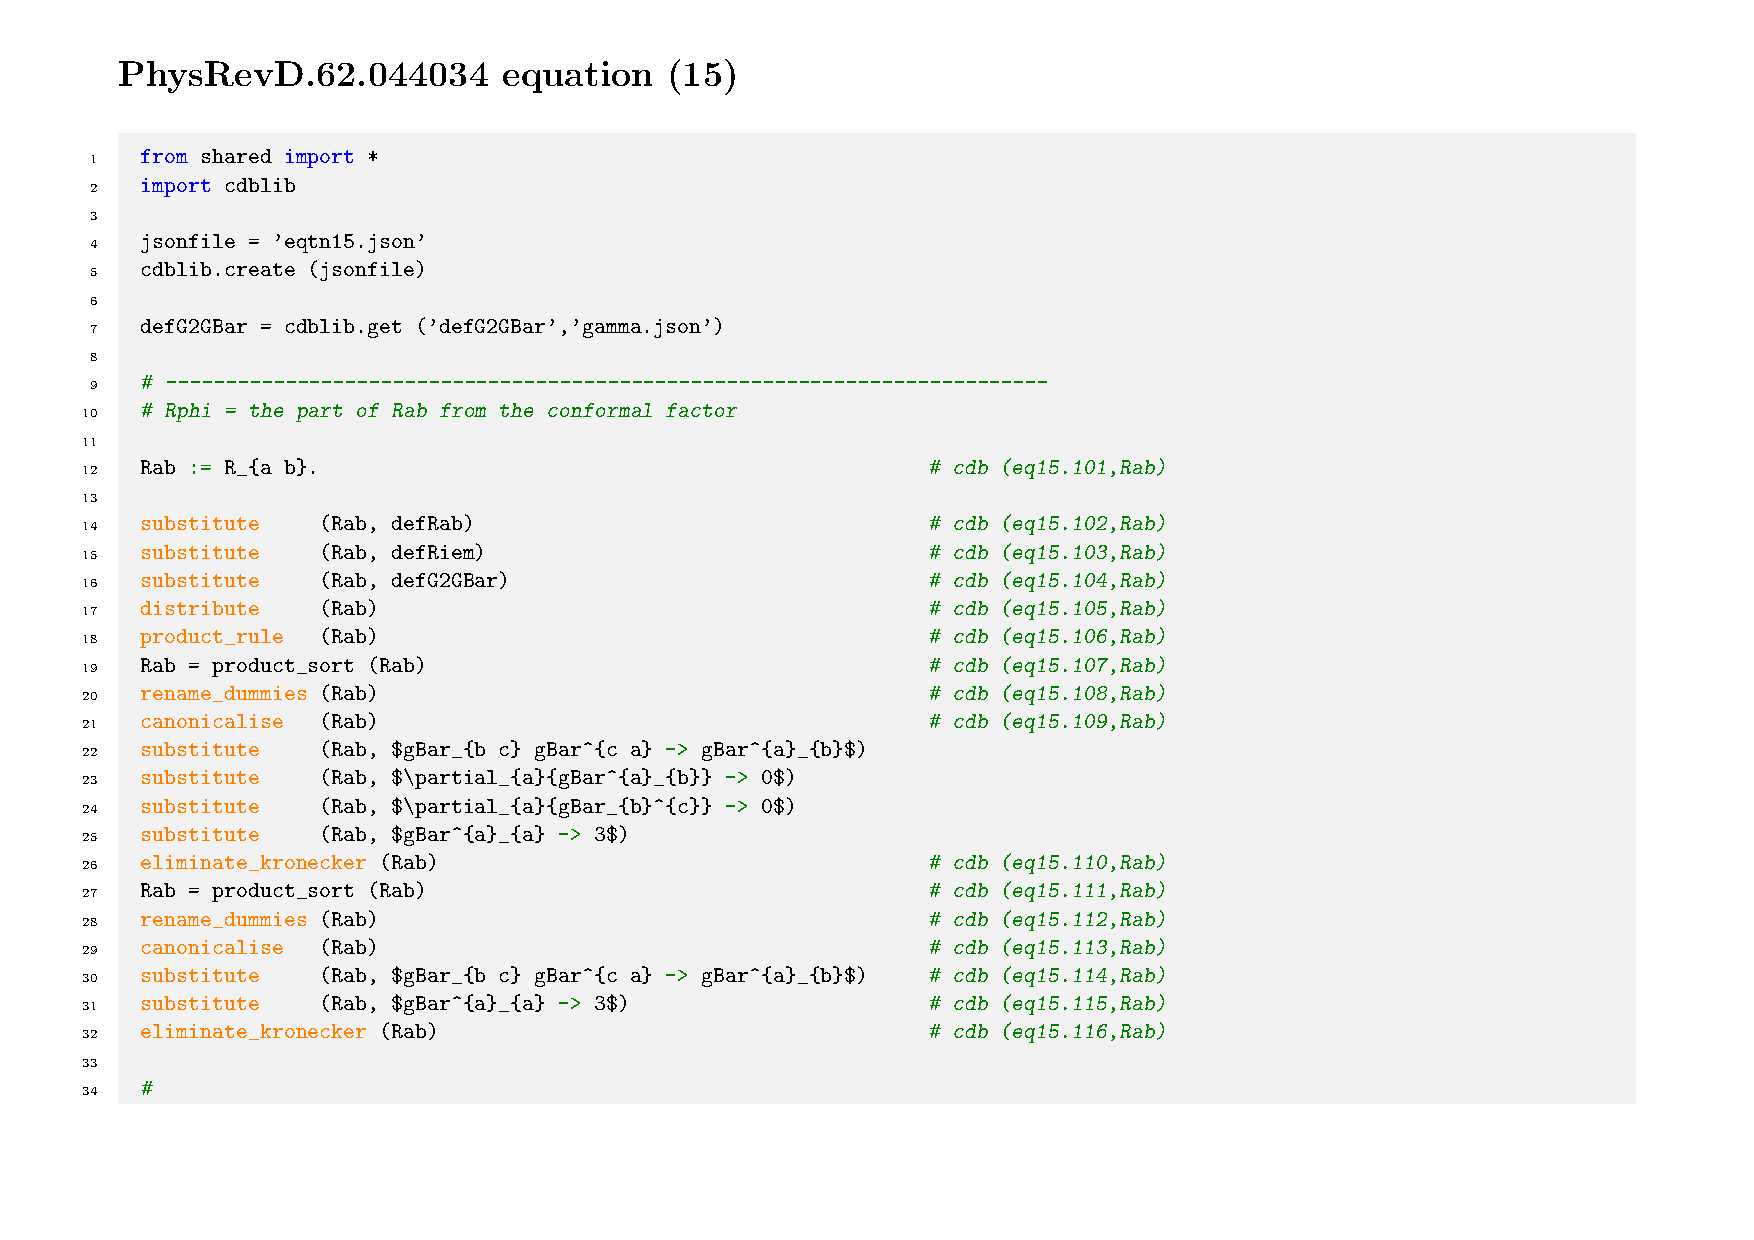
\includepdf[pages=1-]{./eqtn15.pdf}
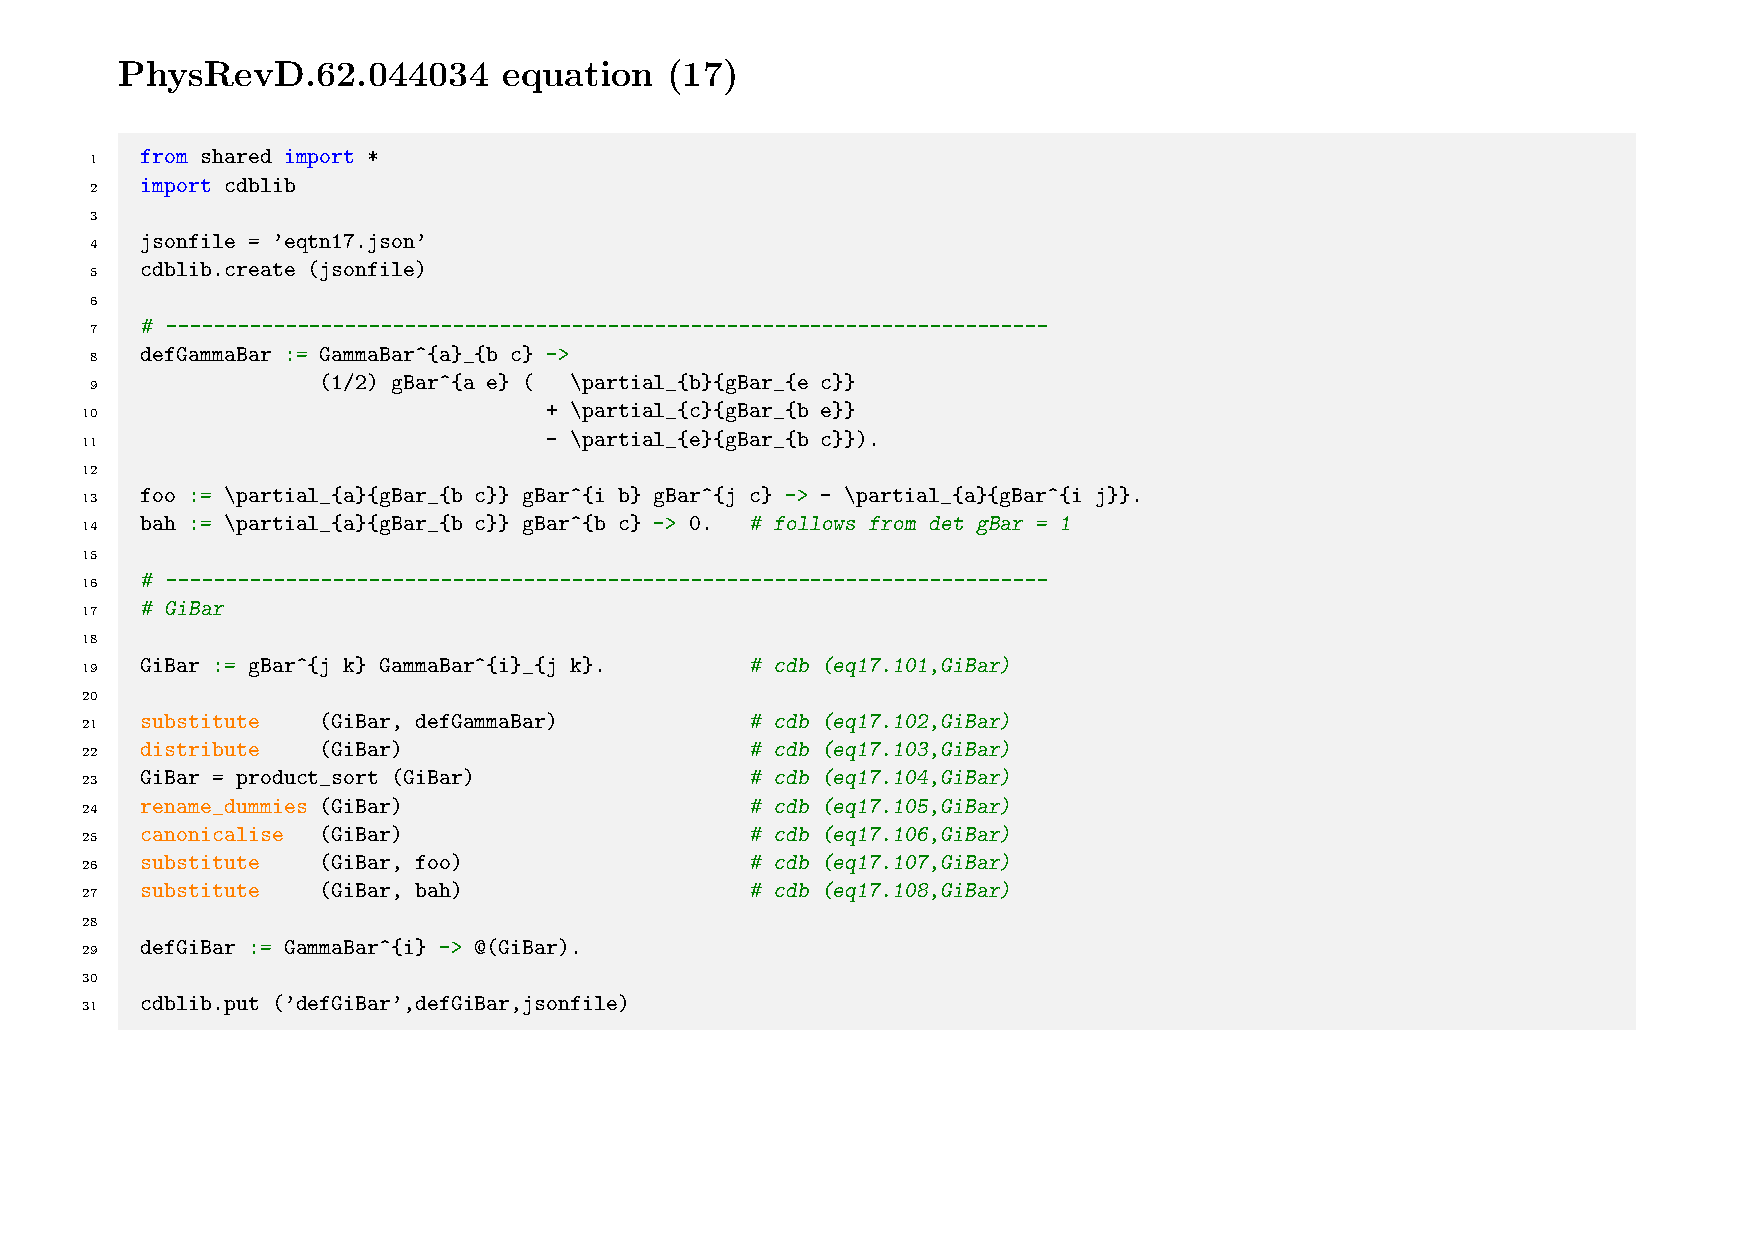
\includepdf[pages=1-]{./eqtn17.pdf}
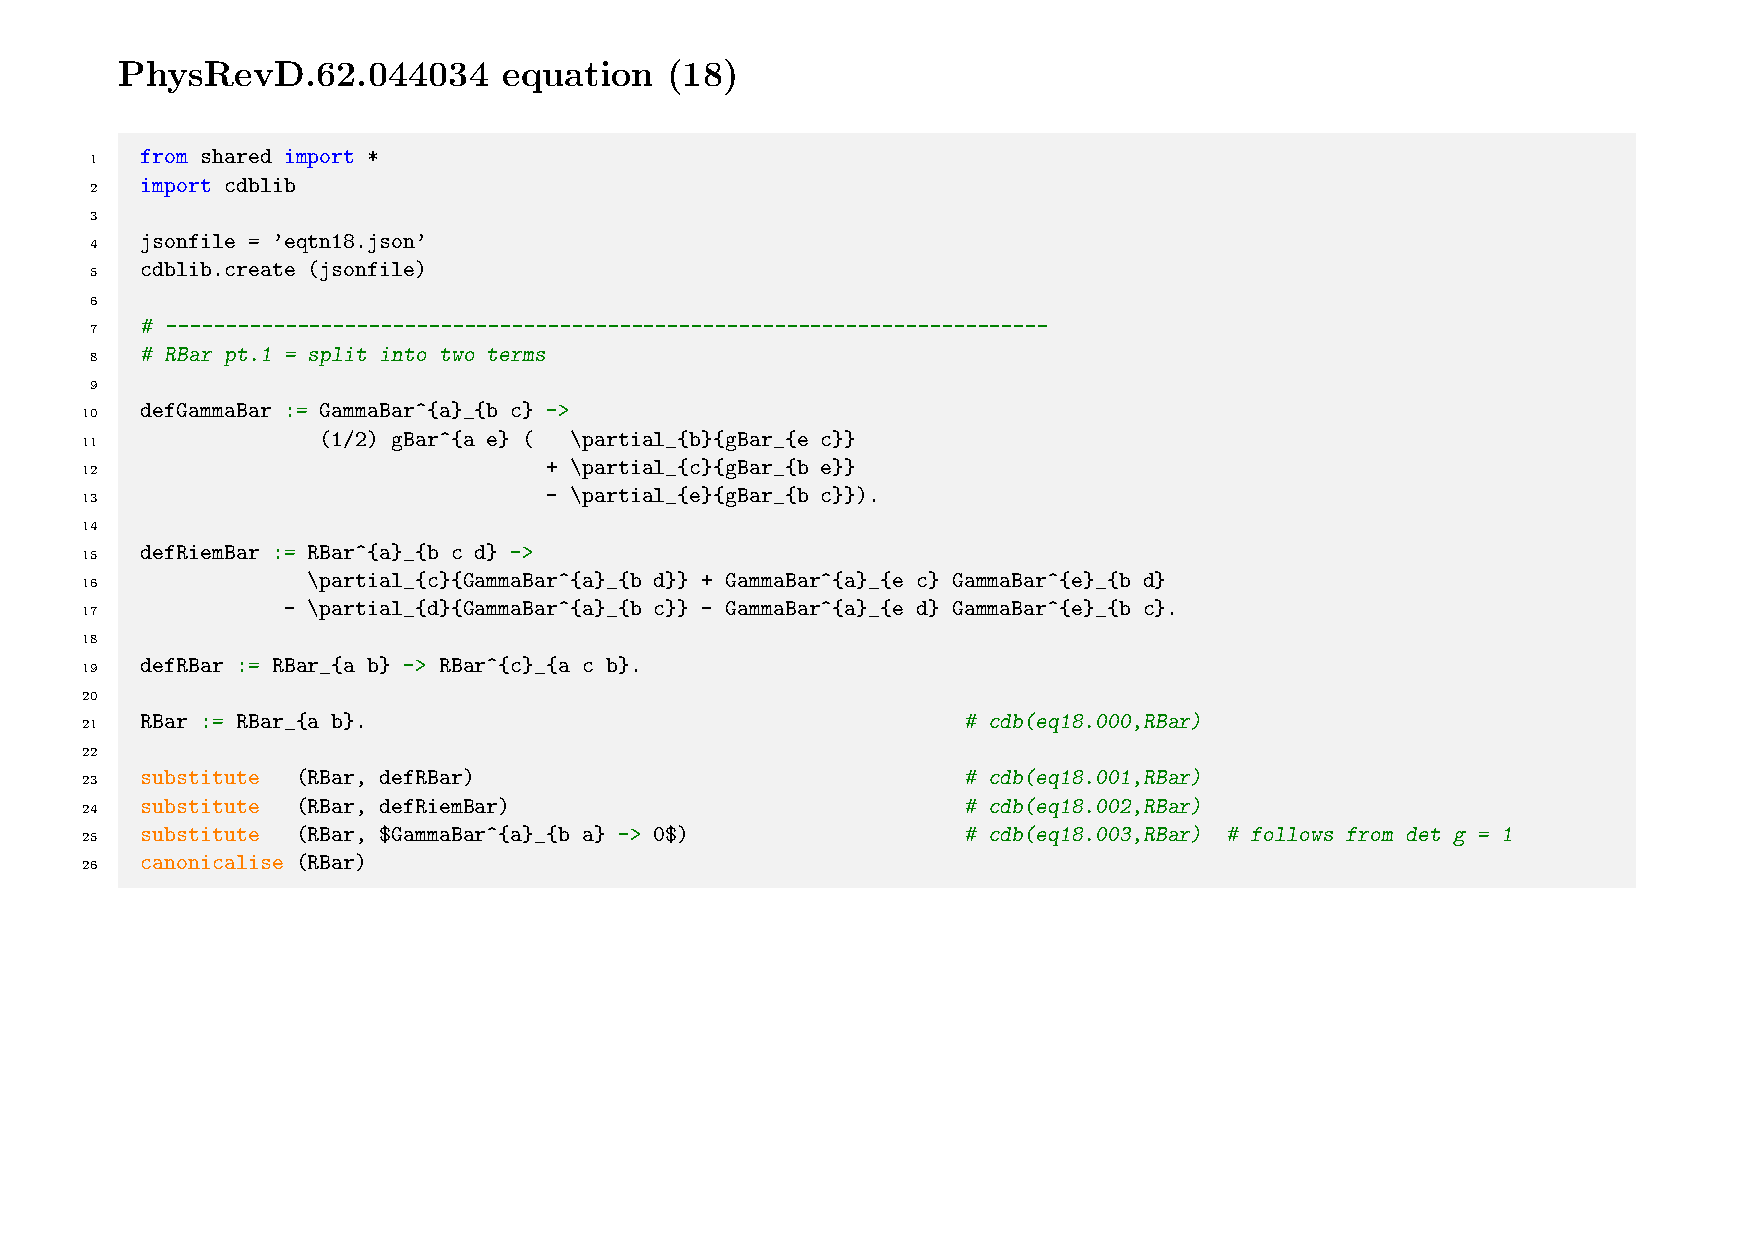
\includepdf[pages=1-]{./eqtn18.pdf}
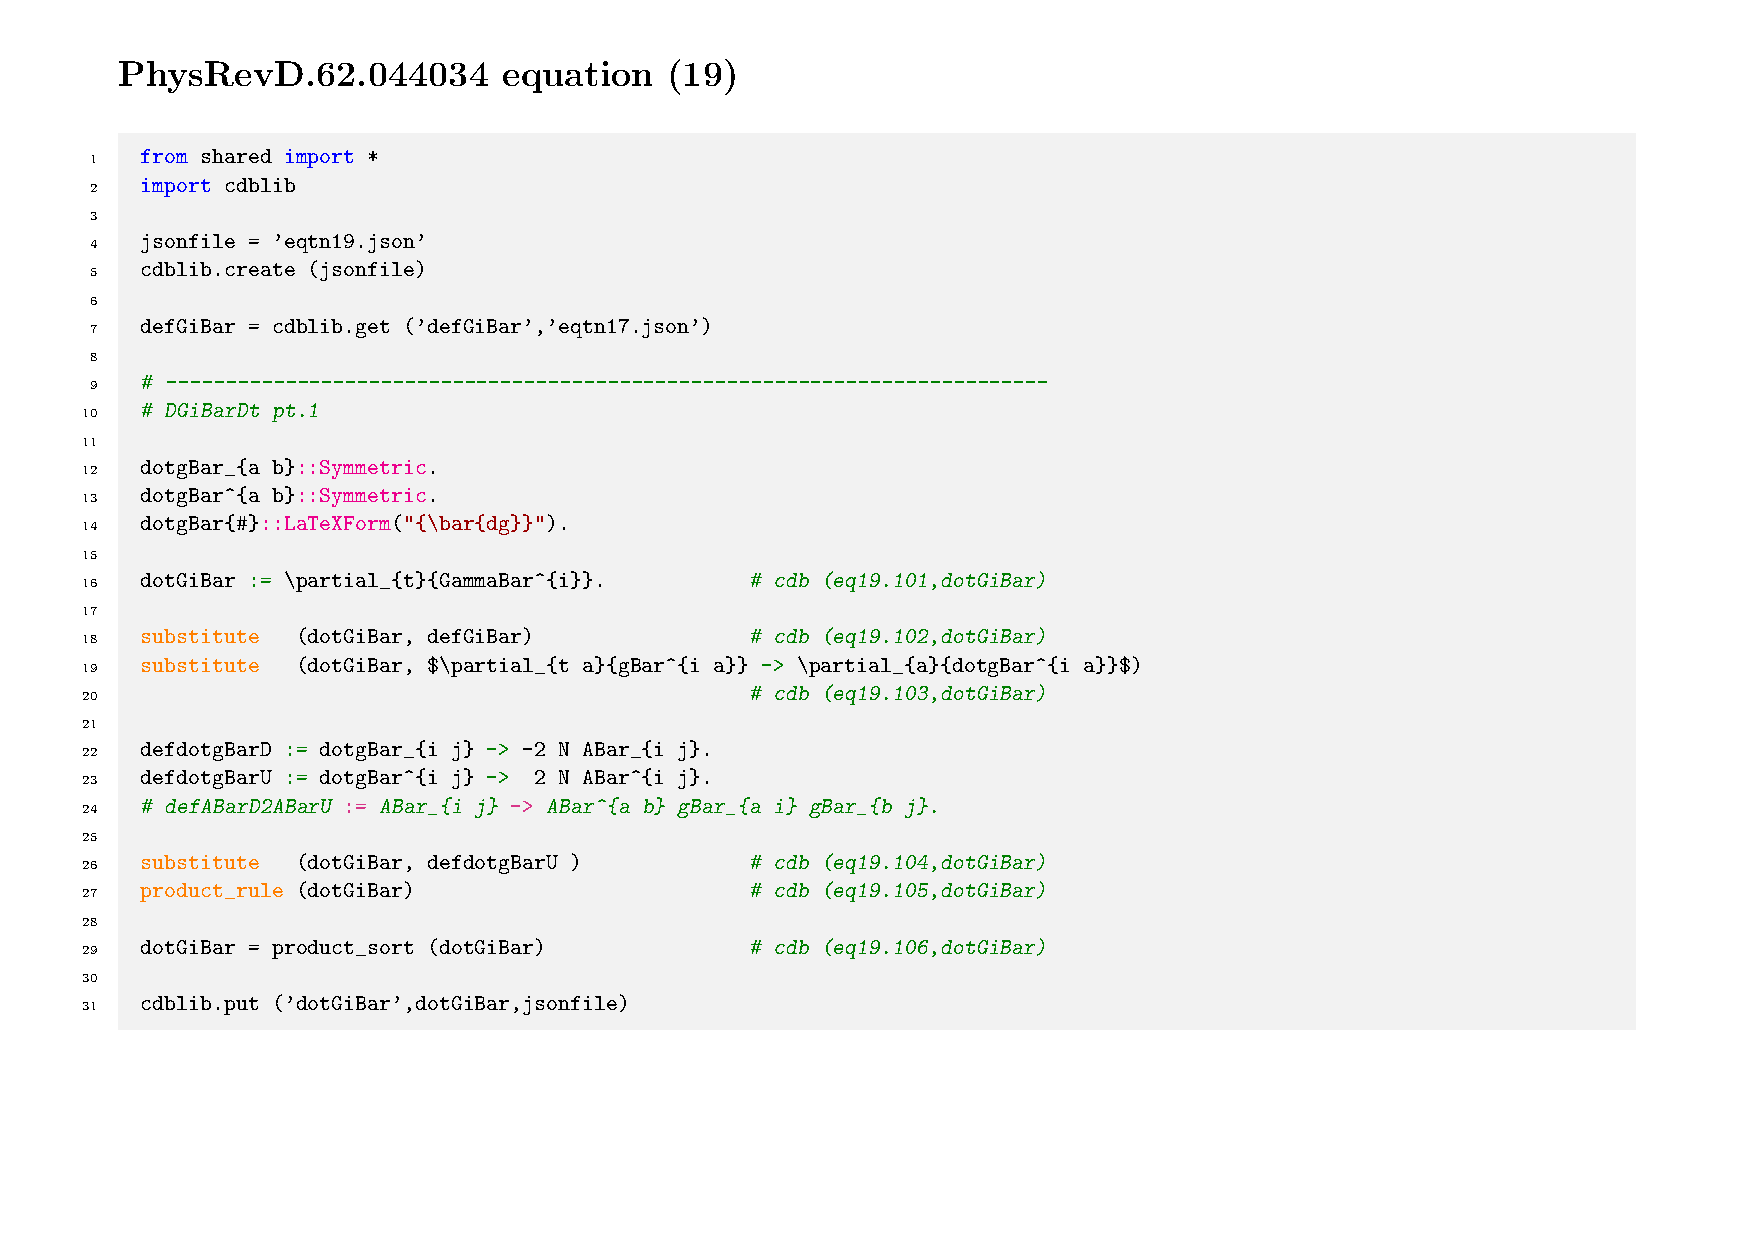
\includepdf[pages=1-]{./eqtn19.pdf}
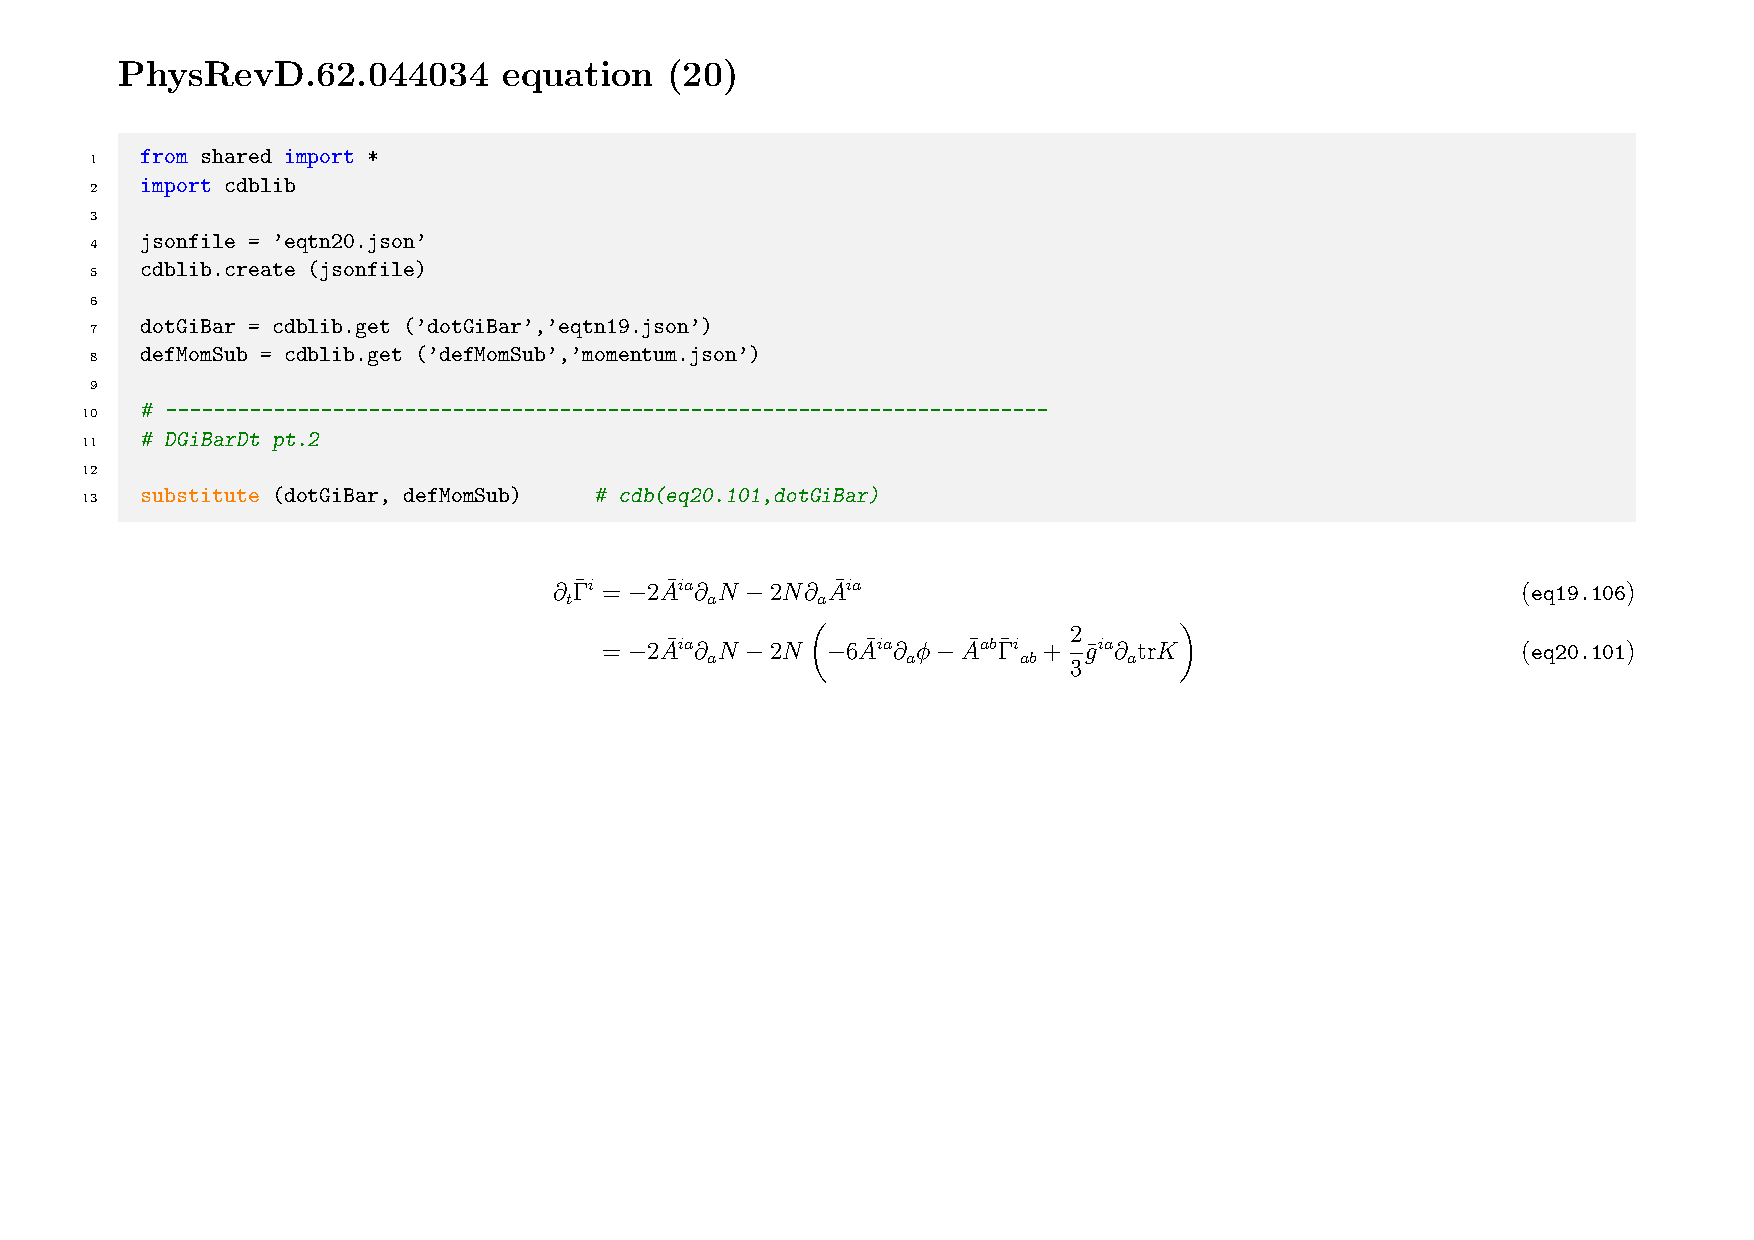
\includepdf[pages=1-]{./eqtn20.pdf}

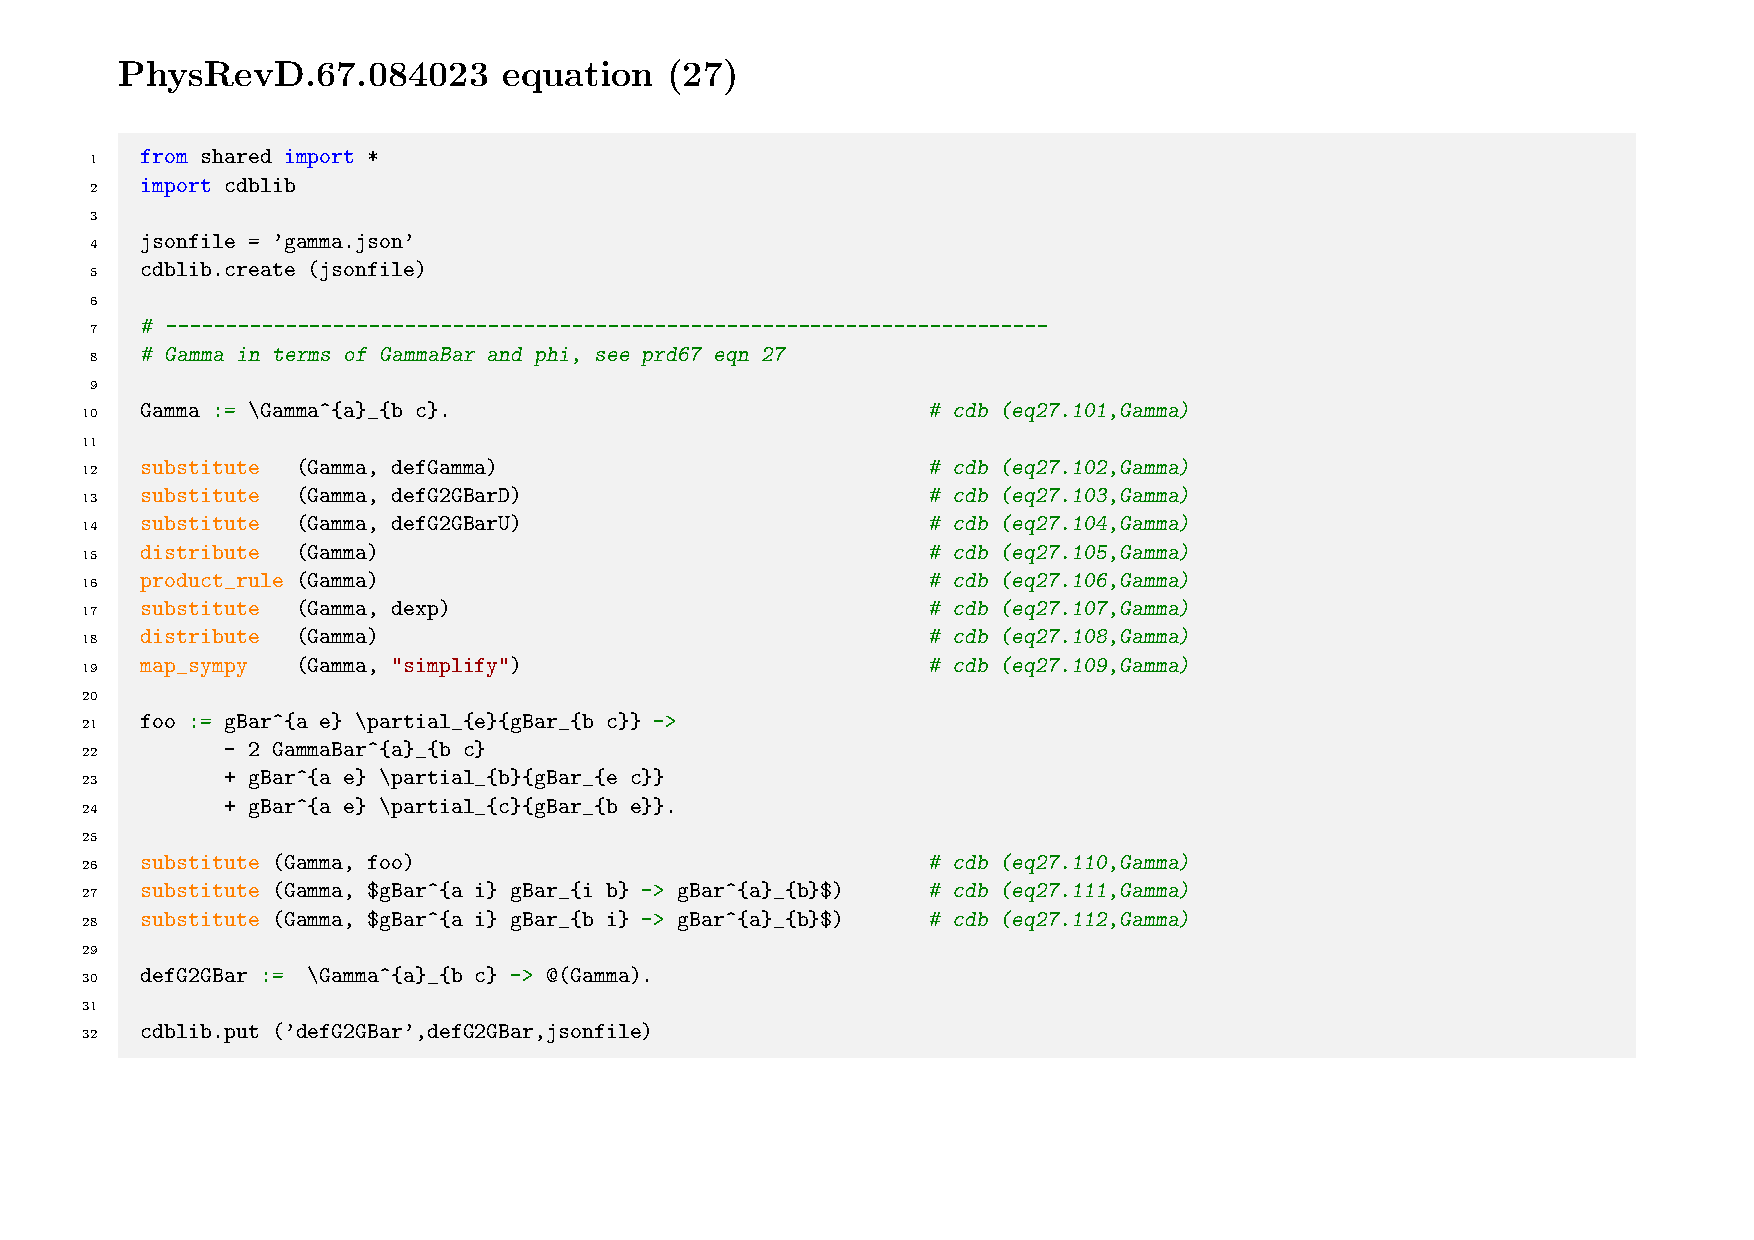
\includepdf[pages=1-]{./gamma.pdf}
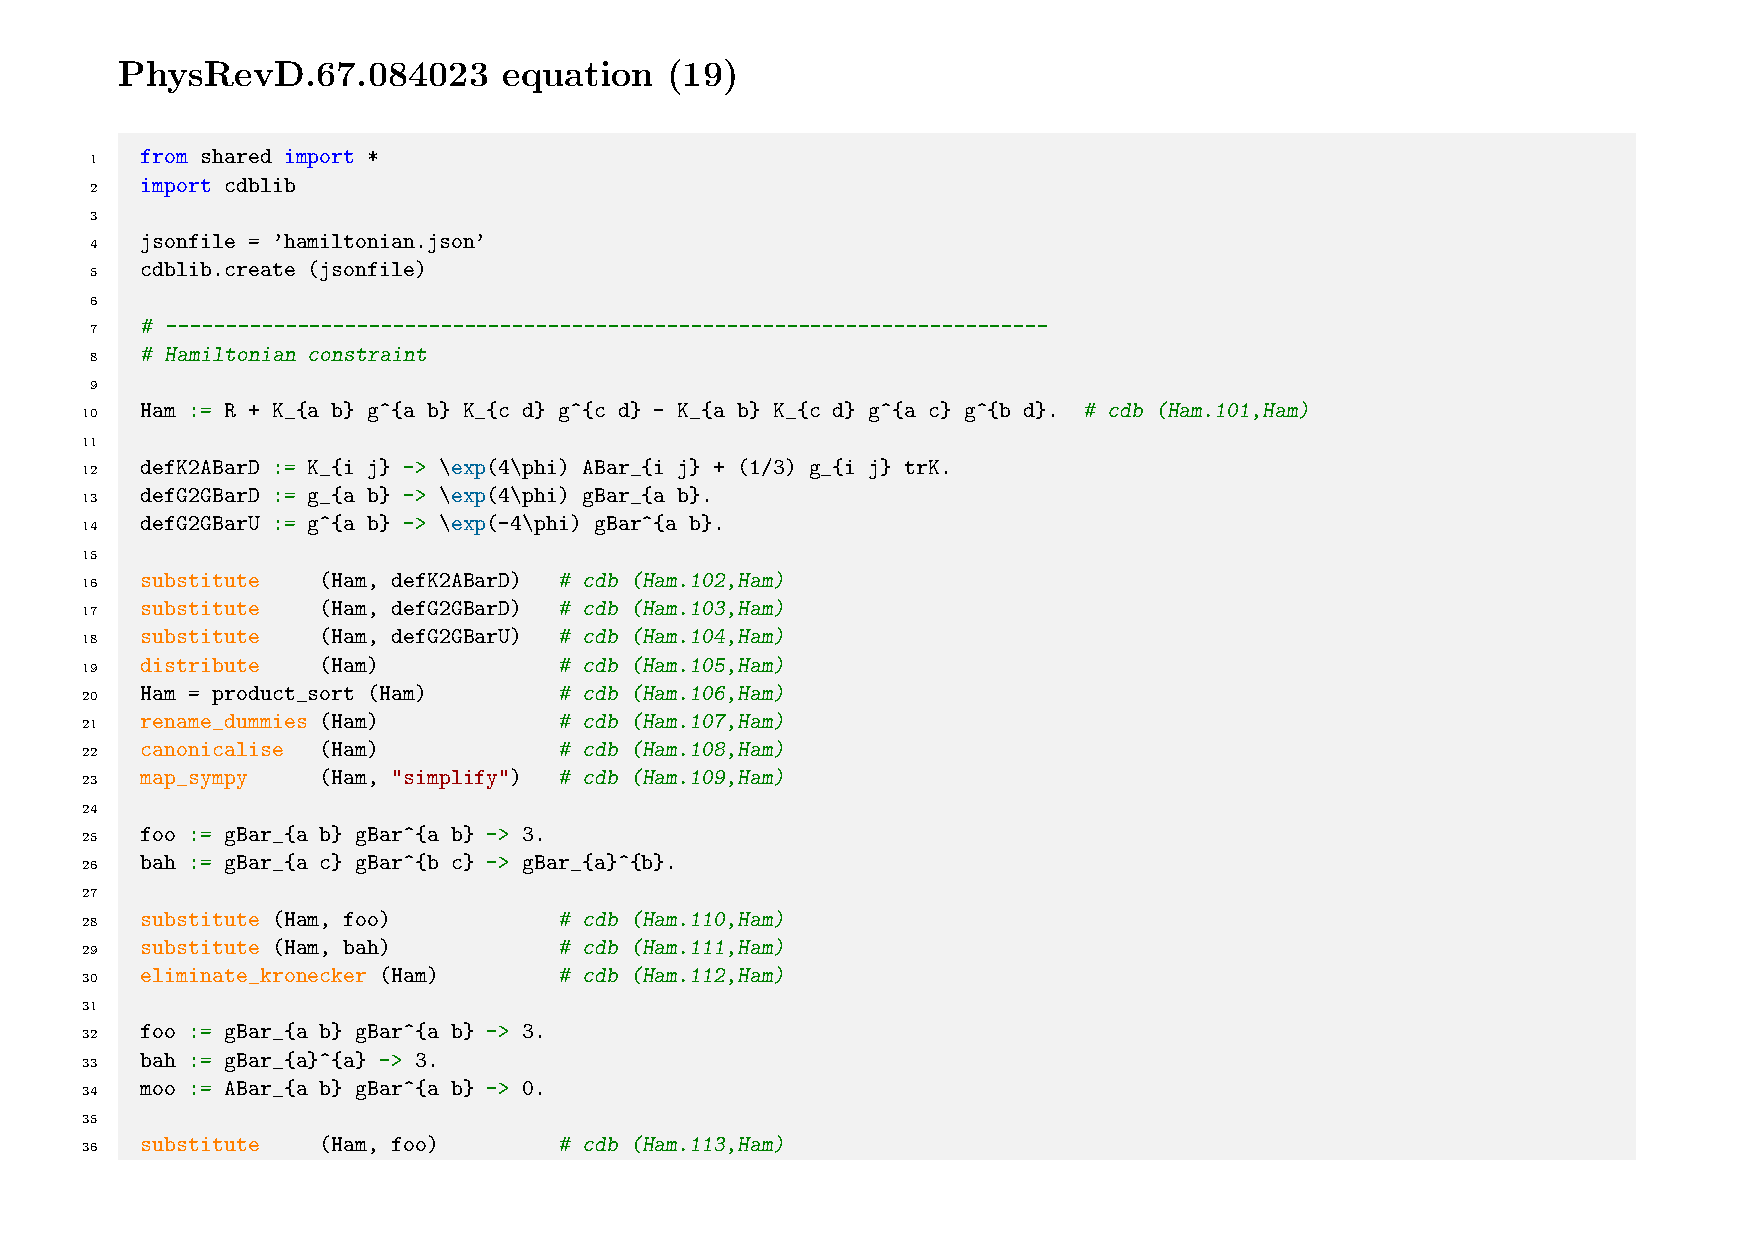
\includepdf[pages=1-]{./hamiltonian.pdf}
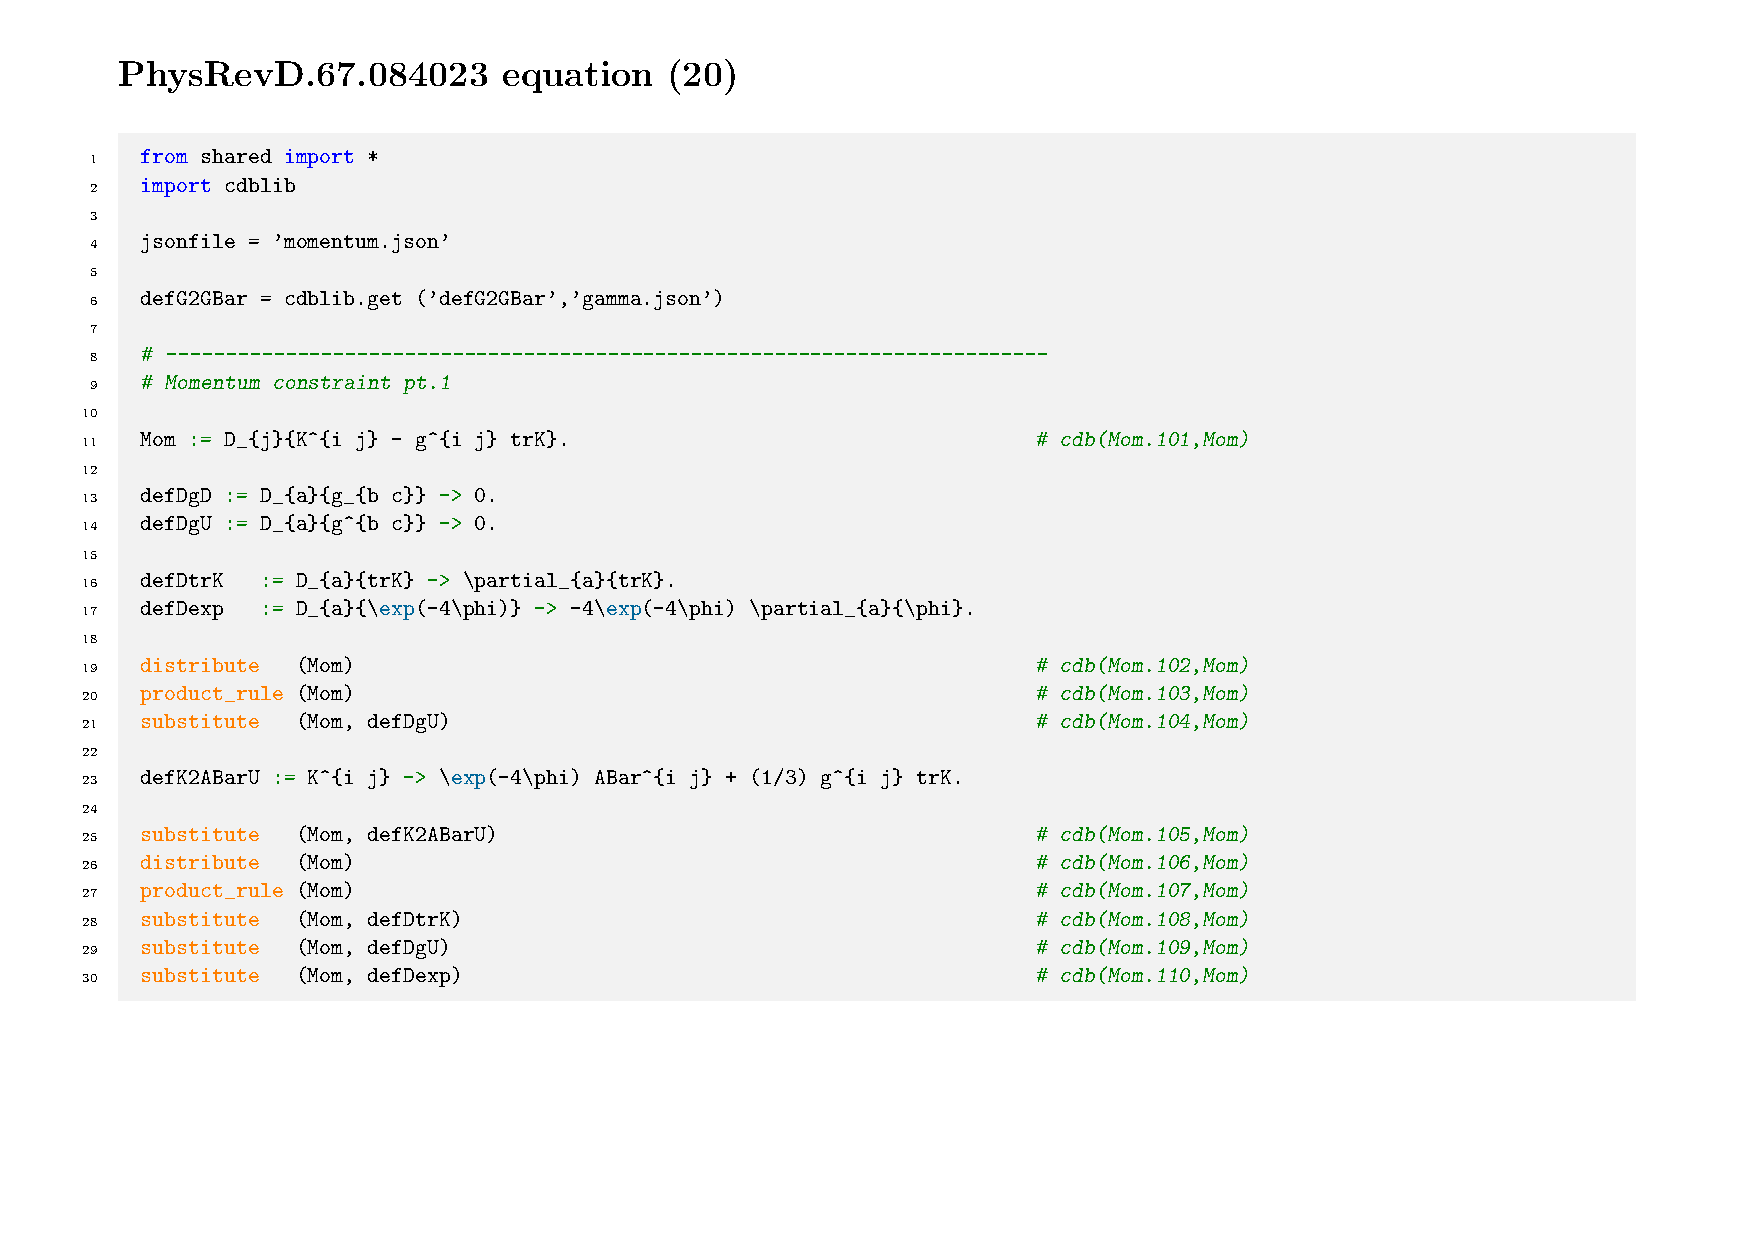
\includepdf[pages=1-]{./momentum.pdf}

\end{document}
